% \documentclass[9pt,a5paper,twoside,dutch,english]{book}                % options used for 'Hoofdstuk' or 'Chapter'
 \documentclass[10pt,a4paper,twoside,dutch,english]{book}
 
%%%%%%%%%%%%%%%%%%%%%%%%%%
%% PACKAGE LOADING TIME %%
%%%%%%%%%%%%%%%%%%%%%%%%%%

\usepackage{siunitx}
%\usepackage{lscape}
\usepackage{gensymb}
\usepackage{pseudocode}
\usepackage{times}      % use Times New Roman Type 1 fonts  (redefines sfdefault,rmdefault,ttdefault)
%\usepackage[T1]{fontenc}
%\usepackage{pslatex}
\usepackage[times]{quotchap}   % fancy chapter beginning
\usepackage{fancyhdr}
%\usepackage[sectionbib]{chapterbib2} % bibliography per chapter
%\usepackage[sectionbib]{chapterbib2} % bibliography per chapter
% (sectionbib -> bibliography is \section* instead of \chapter*), should come before babel chapterbib2 
%because local version is 1.9 and solves bug that header was 'References' instead of Chaptername
\usepackage[dutch,english]{babel}
%\usepackage[sectionbib,numbers,sort&compress]{natbib}  %for citations a la 'Vermeulen et al.' instead of [1]
%\usepackage{tocbibind} % automatically add bibliography, list of figures, ... to table of contents
% \usepackage[a5paper,verbose, asymmetric, centering, top=2.2cm, bottom=1.5cm]{geometry}  % better control over margins
\usepackage[a4paper,verbose, asymmetric, centering, top=3cm, bottom=2.5cm]{geometry}  % better control over margins
%\usepackage[hang]{caption}     %better control over captions (sideways, font, ...)  hang -> 2nd line of caption is indented (caption2 is deprecated and beta)
\usepackage[justification=centering]{caption}     %better control over captions (sideways, font, ...)  
\usepackage{subfigure}  % with scriptsize or so, one can adapt the size
\usepackage{cite}

\usepackage{enumerate}  % to make it possible to define the numbers (A,a, ...)
\usepackage{verbatim}   % extra support for verbatim environments
\usepackage{float}      % you can define 'H' so that floats are forced to be putted 'here'
\usepackage{multirow}   % multirow{nrows}[bigstruts]{width}[fixup]{text} multirow cells
\ifx\pdftexversion\undefined
\usepackage[dvips]{graphicx}
\else
\usepackage[pdftex]{graphicx}
\fi
%\usepackage{psfrag}
%\usepackage{chappg}     % page numbering (chapno-pageno), for ToC
\usepackage{url}        % for better url typesetting
\usepackage{expdlist}   % Expanded description (e.g. better alignement) -> needed for acronym_expdlist package
\usepackage{acronym_expdlist}   % for list of acronyms
\usepackage{hhline}     % generates nicer table lines (without missing pixels) + more flexible
%\usepackage{colortbl}  % for coloured columns
%\usepackage{threeparttable}     % adds the possibility to add footnotes in tables
\usepackage{afterpage}  % adds \afterpage command, which makes it possible to issue \afterpage{\clearpage} which flushes all floats after this page
%\usepackage{amsmath}    % adds extra commands, ao. \text within math environment
\usepackage{amsmath,amsfonts,amsthm}
\usepackage{marvosym}   % for Euro symbol
\usepackage{ifthen}     % ifthenelse command
%\usepackage{mathenv}	% better eqnarray
\usepackage{listings}
\usepackage{setspace}
\usepackage{booktabs}
\def\hrulefill{\leavevmode\leaders\hrule height 1.5pt\hfill\kern 0pt \\}


%%%%%%%%%%%%%%%%%
%% PAGE LAYOUT %%
%%%%%%%%%%%%%%%%%

%%%%%%%%%%%%%%%%%%%%%%%%%%%%%%%%%%%%%%%%%%%%%%%%%%%%%%%%%%%%%%%%%%%%%%
% document: page_layout_definition.tex
%
% last modified: $Id: page_layout_definition.tex,v 1.1 2005/11/18 11:49:23 bvolckae Exp $
%UPDATED ON 05/02/2014 BY SEVENOIS RUBEN TO KEEP COMPATIBILITY WITH NEWER PACKAGE VERSIONS
%
% author: Filip De Turck, Stefaan Vanhastel, Bart Duysburgh, Brecht Vermeulen, Bruno Volckaert, Steven Van den Berghe
%%%%%%%%%%%%%%%%%%%%%%%%%%%%%%%%%%%%%%%%%%%%%%%%%%%%%%%%%%%%%%%%%%%%%%

%%%%%%%%%%%%%%%%%%%%%%%%%%%%%%%%%%%%%%%%%%%%%%%%%%%%%%%%%%%%%%%%%%%%%%

%
% basic dimensions when printing the small page %
% and by using the geometry package             %

% settings Filip en Stefaan
%\geometry{bottom=4.0cm,rmargin=4.25cm,body={12.5cm,19.5cm}} % 10pt op a4
%\geometry{marginpar=0.0cm,marginparsep=0.0cm,twosideshift=0.0cm}

% new settings (according book pim which was approved by the promotors) by Bart Duysburgh
%\geometry{bottom=5.34cm,rmargin=4.5cm,body={11.5cm,18.92cm}} % 10pt op a4
%\geometry{marginpar=0.0cm,marginparsep=0.0cm,twosideshift=0.0cm}

\geometry{body={11.5cm,18.92cm}} % 10pt op a4
% \geometry{bottom=5.34cm,rmargin=4.5cm,body={11.5cm,18.92cm}} % 10pt op a4
\geometry{twoside,marginpar=0.0cm,marginparsep=0.0cm}%,twosideshift=0.0cm}

%\geometry{bottom=2.15cm,rmargin=2.5cm,body={14.14125cm,23.6cm}} % 12pt op a4

%%%%%%%%%%%%%%%%%%%%%%%%%%%%%%%%%%%%%%%

\setlength{\textwidth}{11.5cm}
%\setlength{\textheight}{19.5cm}
%\setlength{\topmargin}{0.0cm}
%\setlength{\oddsidemargin}{0.7cm}
%\setlength{\evensidemargin}{0.7cm}
%\setlength{\marginparwidth}{0pt}
%\setlength{\marginparsep}{0pt}

%%%%%%%%%%%%%%%%%%%%%%%%%%%%%%%%%%%%%%%

\renewcommand{\topfraction}{0.8}

%%%%%%%%%%%%%%%%%%%%%%%%%%%%%%%%%%%%%%%

%%%%%%%%%%%%%%%%%%%%%%%%%%%%%%%%%%%%%%
%% change for subfigure
\renewcommand{\subfigcapskip}{0pt}
%%%%%%%%%%%%%%%%%%%%%%%%%%%%%%%%%%%%%%

%%%%%%%%%%%%%%%%%%%%%%%%%%%%%%%%%%%%%%%
% headings %

\fancypagestyle{plain}{
\fancyhf{}
\renewcommand{\headrulewidth}{0pt}
\renewcommand{\footrulewidth}{0pt}}

\pagestyle{fancy}
\fancyhf{} %clear all header and footer fields
\addtolength{\headwidth}{\marginparsep}
\addtolength{\headwidth}{\marginparwidth}

%\renewcommand{\chaptermark}[1]{\markboth{\chaptername\ \thechapter. \ #1}{}}

\renewcommand{\chaptermark}[1]{\markboth{#1}{}}
%\renewcommand{\sectionmark}[1]{\markright{\thesection\ #1}}

%\newcommand\fdtsvrightmarktmp{{\scshape\small Chapter }}
%\newcommand\fdtsvrightmark{{\scshape\small{Acknowledgment}}}
%\newcommand\fdtsvleftmark{{\scshape\small{Dankwoord}}}

\newcommand\oddpageleftmark{}
\newcommand\evenpagerightmark{}

%\fancyhead[LE,RO]{\itshape\bfseries\small\thepage}
%\fancyhead[LO]{\itshape\bfseries\small\leftmark}
%\fancyhead[RE]{\itshape\bfseries\small\rightmark}
\fancyhead[LE,RO]{\small\thepage}
\fancyhead[LO]{\oddpageleftmark}
\fancyhead[RE]{\evenpagerightmark}
%\fancyfoot[C]{\itshape\bfseries\footnotesize \chaptername\ \thechapter}

%%%%%%%%%%%%%%%%%%%%%%%%%%%%%%%%%%%%%%%%%%%%%%%%%%%%


%%%%%%%%%%%%%%%%%%%%%%%%%%%%%%%%%%%%%%%%%%%%%%%%%%%%
% depth of numbering and depth of table of contents %

\setcounter{tocdepth}{3} % titels tot en met niveau subsubsection worden in table of contents opgenomen
\setcounter{secnumdepth}{3} % tot en met niveau subsubsection wordt er genummerd
%%%%%%%%%%%%%%%%%%%%%%%%%%%%%%%%%%%%%%%%%%%%%%%%%%%



%%%%%%%%%%%%%%%%%%%%%%%%%%%%%%%%%%%%%%%%%%%%%%%%%%%
%%%%% Definition for Big letter at the beginning of a paragraph %%
\def\PARstart#1#2{\begingroup\def\par{\endgraf\endgroup\lineskiplimit=0pt}
    \setbox2=\hbox{\uppercase{#2} }\newdimen\tmpht \tmpht \ht2
    \advance\tmpht by \baselineskip\font\hhuge=cmr10 at \tmpht
    \setbox1=\hbox{{\hhuge #1}}
    \count7=\tmpht \count8=\ht1\divide\count8 by 1000 \divide\count7 by\count8
    \tmpht=.001\tmpht\multiply\tmpht by \count7\font\hhuge=cmr10 at \tmpht
    \setbox1=\hbox{{\hhuge #1}} \noindent \hangindent1.05\wd1
    \hangafter=-2 {\hskip-\hangindent \lower1\ht1\hbox{\raise1.0\ht2\copy1}%
    \kern-0\wd1}\copy2\lineskiplimit=-1000pt}
%%%%%%%%%%%%%%%%%%%%%%%%%%%%%%%%%%%%


%%%%%%%%%%%%%%%%%%%%%%%%%%%%%%%%%%%%%%%%%%%%%%%%%%%%
%%% Nog een paar andere zaken  %%%%
%% om een cross-ref naar een voetnoot te kunnen maken definier ik \usefn %%
\newcommand{\usefn}[1]{\mbox{\textsuperscript{\normalfont#1}}}

%\setlength{\captionindent}{1cm}
\renewcommand{\captionfont}{\small \itshape \mdseries \rmfamily}
\renewcommand{\subcapsize}{\footnotesize \itshape \mdseries \rmfamily}

\AtBeginDocument{%
%   \renewcommand{\figurename}{Fig.}%
%   \renewcommand{\tablename}{TABLE}%
   \renewcommand{\tablename}{Table}
   \renewcommand{\bibname}{References}%
}

%%%%%%%%%%%%%%%%%%%%%%%%%%%%%%%%%%%%%%%%%%%%%%%%%%%


% \setlength{\parindent}{0cm}             % Inspringen van eerste lijn van paragrafen is niet gewenst.

%%%%%%%%%%%%%%%%%
%% HYPHENATION %%
%%%%%%%%%%%%%%%%%

\hyphenation{} % to have a separate file with hyphenations

%%%%%%%%%%%%%%%%%%%%
%%  START BOOK    %%
%%%%%%%%%%%%%%%%%%%%

\usepackage[pagewise]{lineno}
\linenumbers

\begin{document}
\graphicspath{{fig/}}
\restylefloat{figure}
\restylefloat{table}
\newfloat{algorithm}{ht}{alg}

%%   FRONT PAGE       %%
%%%%%%%%%%%%%%%%%%%%%%%%
% 
 \thispagestyle{empty}   % no headings for this page
% 
% % Header
 \noindent
 \begin{minipage}{3cm}%
   \includegraphics*[width=6cm]{/home/isa/ownCloud/DOCTORAAT/info/logos/VUBlogo}
 \end{minipage}\hfill
 \begin{minipage}{8cm}
 \raggedleft
 \textsf{Vrije Universiteit Brussel\\ \vspace{.15cm}
 Faculteit Wetenschappen en\\
 Bio-ingenieurswetenschappen\\  \vspace{.15cm}
 Departement Natuurkunde}
 \end{minipage}
% 
% % Title
\begin{center}
% \vspace{1.3cm}
\vspace{5cm}
\bigskip
 \hrulefill \vspace{.2cm}
 \onehalfspacing
     \LARGE \noindent \textsf{Search for Dark Matter in the Monojet\\ and Trackless Jets Final States with \\the CMS Detector at the LHC}\\ 
 \hrulefill 
% \vspace{.5cm}
\vspace{1cm}
 \bigskip
   \Large\noindent \textsf{Isabelle De Bruyn} \\
 \bigskip
 \large
% \vspace{1.8cm}
\vspace{2.5cm}
\textsf{Promotor\\ \vspace{.1cm}
Prof. Dr. Steven Lowette}
 \normalsize
% % Footer
 \vfill
 \textsf{Proefschrift ingediend met het oog op het behalen van de\\ academische graad van Doctor in de Wetenschappen\\ \vspace{.3cm}
 September 2017}\
 
 \end{center}

\clearpage{\pagestyle{empty}\cleardoublepage}

%% ACKNOWLEDGMENT   %%
%%%%%%%%%%%%%%%%%%%%%%%

\selectlanguage{dutch}
\hyphenation{bu-reau-ge-no-ten}
\frontmatter
\chapter{Acknowledgements}
\vspace{0.35in}

% dankwoord...

% "I am very much indebted to my friend the APVe; without him, there would have been so much more buffer overflow and coherent noise"

% \begin{flushright}{\emph{Brussel, maand 2017\\
% Isabelle De Bruyn}}
% \end{flushright}
% \selectlanguage{english}

\clearpage{\pagestyle{empty}\cleardoublepage}

%%   TOC, LIST OF FIGURES, LIST OF TABLES, ACRONYMS     %%
%%%%%%%%%%%%%%%%%%%%%%%%%%%%%%%%%%%%%%%%%%%%%%%%%%%%%%%%%%

\renewcommand{\contentsname}{Table of Contents} % original name = Contents

\tableofcontents
\clearpage{\pagestyle{empty}\cleardoublepage}

% 	%% SUMMARY IN DUTCH       %%
% %%%%%%%%%%%%%%%%%%%%%%%%%%%%
% \selectlanguage{dutch}
% \graphicspath{{chapt_dutch/}{chapt2/}{chapt3/}{chapt4/}}
\renewcommand{\thesection}{\arabic{section}}    % chapter without number, so don't use chapterno.sectionno

\renewcommand{\bibname}{Referenties}
% Header
\renewcommand\evenpagerightmark{{\scshape\small Nederlandse Samenvatting}}
\renewcommand\oddpageleftmark{{\scshape\small Summary in Dutch}}

\chapter[Nederlandse samenvatting]%
{Nederlandse samenvatting \\\makebox[2.82in]{--Summary in Dutch--}}

\hyphenation{job-respons-tijd blijkt dynami-sche mo-nitoringarchitectuur monito-ringplatform service-manager verde-ling reke-ning orga-nisatieprofielen resource-interconnec-ties}
\def\hyph{-\penalty0\hskip0pt\relax}

nederlandse samenvatting

\clearpage

\bibliographystyle{phdbib}
\bibliography{PhD}

\clearpage{\pagestyle{empty}\cleardoublepage}

\renewcommand*{\thesection}{\thechapter.\arabic{section}}       % reset again to chaptnum.sectnum



% \selectlanguage{english}
% \graphicspath{{chapt_dutch/}{chapt2/}{chapt3/}{chapt4/}}
\renewcommand{\thesection}{\arabic{section}}    % chapter without number, so don't use chapterno.sectionno

\renewcommand{\bibname}{References}
% Header
\renewcommand\evenpagerightmark{{\scshape\small English summary}}
\renewcommand\oddpageleftmark{{\scshape\small English summary}}

\chapter[English summary]%
{English summary}

\hyphenation{}
%\def\hyph{-\penalty0\hskip0pt\relax}

insert english summary here...

\clearpage

\bibliographystyle{phdbib}
\bibliography{PhD}

\clearpage{\pagestyle{empty}\cleardoublepage}

\renewcommand*{\thesection}{\thechapter.\arabic{section}}       % reset again to chaptnum.sectnum




%% THE BOOK ITSELF   %%
%%%%%%%%%%%%%%%%%%%%%%%
\mainmatter     % related to chappg numbering
\selectlanguage{english}
\renewcommand*{\thesection}{\thechapter.\arabic{section}}

\newcommand\fdtsvrightmarktmp{{\scshape\small Chapter }}
\renewcommand\evenpagerightmark{{\scshape\small\chaptername\ \thechapter}}
\renewcommand\oddpageleftmark{{\scshape\small\leftmark}}

%\addtolength{\headwidth}{\marginparsep}
%\addtolength{\headwidth}{\marginparwidth}

%\newcommand{\tm}[1]{$\mbox{#1}^{\mbox{\emph{\scriptsize TM}}}$}

\baselineskip 13.0pt

\graphicspath{{chapt_dutch/}{intro/}{chapt2/}{chapt3/}{chapt4/}}

% Header
\renewcommand\evenpagerightmark{{\scshape\small Introduction}}
\renewcommand\oddpageleftmark{{\scshape\small Introduction}}

%\renewcommand{\bibname}{References}

\hyphenation{}

\chapter{Introduction}

%% Introduction
%%%%%%%%%%%%%%%

\clearpage

%\renewcommand*{\thesection}{\thechapter.\arabic{section}}       % reset again to chaptnum.sectnum

\clearpage{\pagestyle{empty}\cleardoublepage}

\graphicspath{{chapt_dutch/}{intro/}{chapt2/}{chapt3/}{chapt4/}{chapt5/}}

% Header
\renewcommand\evenpagerightmark{{\scshape\small The CMS Detector}}
\renewcommand\oddpageleftmark{{\scshape\small Chapter 2}}

%\renewcommand{\bibname}{References}

\hyphenation{}

\chapter{Dark Matter Scenarios Beyond the Standard Model}
\label{ch2}

\section{The Standard Model of Particle Physics}

\subsection{Elementary particles and their interactions}

\subsection{Unanswered questions of the Standard Model}
\section{Dark matter}

\subsection{Observational evidence}

\subsection{Detection of dark matter}

\subsection{Dark matter models}


\section{Strongly Interacting Massive Particles}

\subsection{Motivation}

\subsection{Experimental constraints}

\clearpage{\pagestyle{empty}\cleardoublepage}

\graphicspath{{chapt_dutch/}{intro/}{chapt2/}{chapt3/}{chapt4/}{chapt5/}}

% Header
\renewcommand\evenpagerightmark{{\scshape\small Chapter 3}}
\renewcommand\oddpageleftmark{{\scshape\small The LHC and the CMS Detector}}

\hyphenation{}

\chapter{The LHC and the CMS Detector}
\label{ch3}

In order to investigate the currently unsolved mysteries of particle physics, such as the existence of dark matter, many experiments can be conducted, among other things at particle colliders. The largest particle accelerator in the world is the \ac{LHC}, located at the \ac{CERN} in Geneva, Switzerland. At this accelerator, protons are being accelerated at energies up to \SI{6.5}{TeV}, giving rise to a record center-of-mass energy of \SI{13}{TeV} in the proton collisions. Using data from the collisions generated at the interaction points along the accelerator ring, the Standard Model can be tested in many ways and searches for particles beyond the Standard Model can be performed. 

In Section~\ref{sec:lhc} more details are given about the \ac{LHC} and the 4 main experiments situated at the interaction points. In particular, the general-purpose \ac{CMS} detector is described in Section~\ref{sec:CMS}.

\section{The Large Hadron Collider at CERN} 
\label{sec:lhc}

The \ac{LHC} was built in the already existing \ac{LEP} collider tunnel, which was excavated in the 1980's and has a circumference of 27.6~km. Contrary to the \ac{LEP} collider, the \ac{LHC} accelerates particles of the same charge, namely protons or lead ions. Much higher luminosities can therefore be reached, since only particles are used and the generation of anti-particles is not needed. Additionally, the colliding particles are not the protons or ions, but their constituents, which carry a varying fraction of the total momentum. %and thus cover a wide energy range. 
This makes the \ac{LHC} the ideal instrument to explore a wide energy range.

\subsection{The LHC injector chain}

The protons (or lead ions) can not directly be injected in the \ac{LHC}, but need to be accelerated gradually in several pre-accelerators, as illustrated in Figure~\ref{fig:accelerators}. For the proton beams, the \ac{LHC} injection chain starts at a bottle of hydrogen, where protons are stripped from the hydrogen atoms and accelerated up to \SI{50}{MeV} by a linear accelerator (LINAC2). The protons are then transfered to a chain of circular accelerators, starting with the \ac{PSB} which accelerates them to an energy of \SI{1.4}{GeV}. Next, the protons go through the \ac{PS} and are delivered to the \ac{SPS} at an energy of \SI{26}{GeV}. Finally, the protons are injected in the \ac{LHC} in opposite direction with an energy of \SI{450}{GeV}. 
% In the \ac{LHC} the protons are then accelerated to \SI{3.5}{TeV} (in 2010 and 2011) or \SI{4}{TeV} (in 2012) during Run 1, and to \SI{6.5}{TeV} during Run 2 (since 2015).

The lead ions are first accelerated in a different linear accelerator, LINAC3, before being injected in the \ac{LEIR} at an energy of \SI{4.5}{MeV} per nucleon. Here the ions are accelerated to an energy of \SI{72}{MeV} per nucleon, and they then follow the same path as the protons through the \ac{PS}, where they are accelerated to \SI{5.9}{GeV} and stripped from the last of their electrons, and the \ac{SPS}, where they are accelerated to \SI{177}{GeV}. The record center-of-mass energy for heavy ion collisions at the \ac{LHC} so far has been \SI{5.02}{TeV} and \SI{8.16}{TeV}, for lead-lead (Pb-Pb) and proton-lead (p-Pb) collisions in 2015 and 2016, respectively.

\begin{figure}[ht]
  \centering
 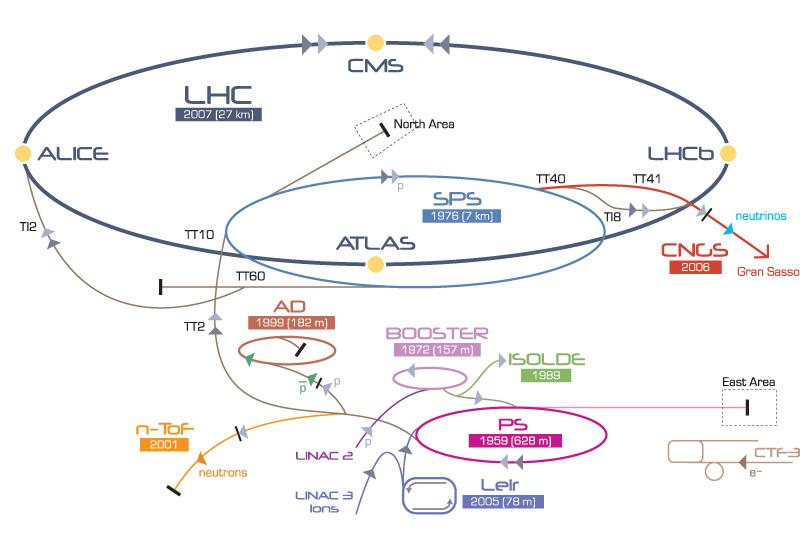
\includegraphics[width=.75\textwidth]{lhc_complex}
 \caption{Schematic view of the various linear and circular accelerators of the \ac{CERN} accelerator complex, including the \ac{LHC} injection chain.}
 \label{fig:accelerators}
\end{figure}

\subsection{The Large Hadron Collider}

The most relevant specifications for a particle physics accelerator are the maximum energy and the luminosity that can be reached. High energy is necessary in order to be able to create new heavy particles, which are for example predicted in many theories beyond the Standard Model.

The protons are kept on the correct orbit by the 1232 \ac{LHC} dipole magnets. These magnets are cooled down to 1.9 K with liquid Helium and supplied with a current of 12~kA to reach the design field of 8.33~T. This limits the maximum beam momentum of the accelerator to 
\begin{equation}
 p = B/\rho = 8.33\, \mathrm{T}/2804\,\mathrm{m}=7\,\mathrm{TeV/c},
\end{equation}
with $\rho$ the bending radius of the tunnel. The protons are accelerated up to the desired energy by \ac{RF} cavities, which produce an oscillating electromagnetic field. As a consequence, late or early protons will feel an acceleration or deceleration, respectively.

A high event rate or luminosity~$\mathcal{L}$ is equally important, to obtain a sufficiently high number of collisions. For a process with cross section $\sigma$, this rate is 
\begin{equation}
 \frac{dN}{dt} = \mathcal{L}\sigma .
\end{equation}
In order to achieve the high design luminosity of $10^{34}$ cm$^{-2}$s$^{-1}$in the \ac{LHC}, the protons are focused in bunches with a \SI{25}{ns} spacing by strong quadrupole magnets around the interaction regions. Additionally, 2\SI{25}{ns} gaps are present as well between the bunch trains, corresponding to the rise time of the injection kicker magnets. One gap of 3~$\mu$s is necessary as well to allow clean beam dumps. These requirements limit the number of bunches to a maximum of 2808.

% Additionally, over 8000 higher-order multipole and corrector magnets focus and stabilize the proton beams.

After almost 25 years of design and construction, the \ac{LHC} was completed in 2008 and the commissioning of the machine started. However, during a powering test on 19 September of the same year an electric arc developed inside a bus bar which led to a large release of helium and a pressure wave that caused extensive mechanical damage to the affected LHC sector. This incident delayed the first collisions, at a beam energy of \SI{900}{GeV}, until late 2009. During 2010 and 2011 a center-of-mass energy of \SI{7}{TeV} was used for the collisions, which was then increased to \SI{8}{TeV} in 2012. The instantaneous luminosity was also increased, starting from $2 \times 10^{32}$ cm$^{-2}$s$^{-1}$ in 2010 to more than $6 \times 10^{33}$ cm$^{-2}$s$^{-1}$ in 2012. During the 3 years of data-taking in Run~1, data corresponding to an integrated luminosity of 45.0~pb$^{-1}$, 6.1~fb$^{-1}$, and 23.3~fb$^{-1}$, respectively, were delivered. After Run~1, a long shutdown (LS1) of 2 years followed, which was used to correct the problems that were discovered in the aftermath of the incident at the startup in 2008, and to upgrade and consolidate the experiments located on the \ac{LHC} ring.

In 2015, the \ac{LHC} restarted operations with Run~2, at an even higher center-of-mass energy of \SI{13}{TeV}. During 2016 the design luminosity of $10^{34}$ cm$^{-2}$s$^{-1}$ was exceeded and a total of 41~fb$^{-1}$ of data were delivered. A comparison of the delivered integrated luminosity per year is shown in Figure~\ref{fig:lumi}.

\begin{figure}[ht]
  \centering
 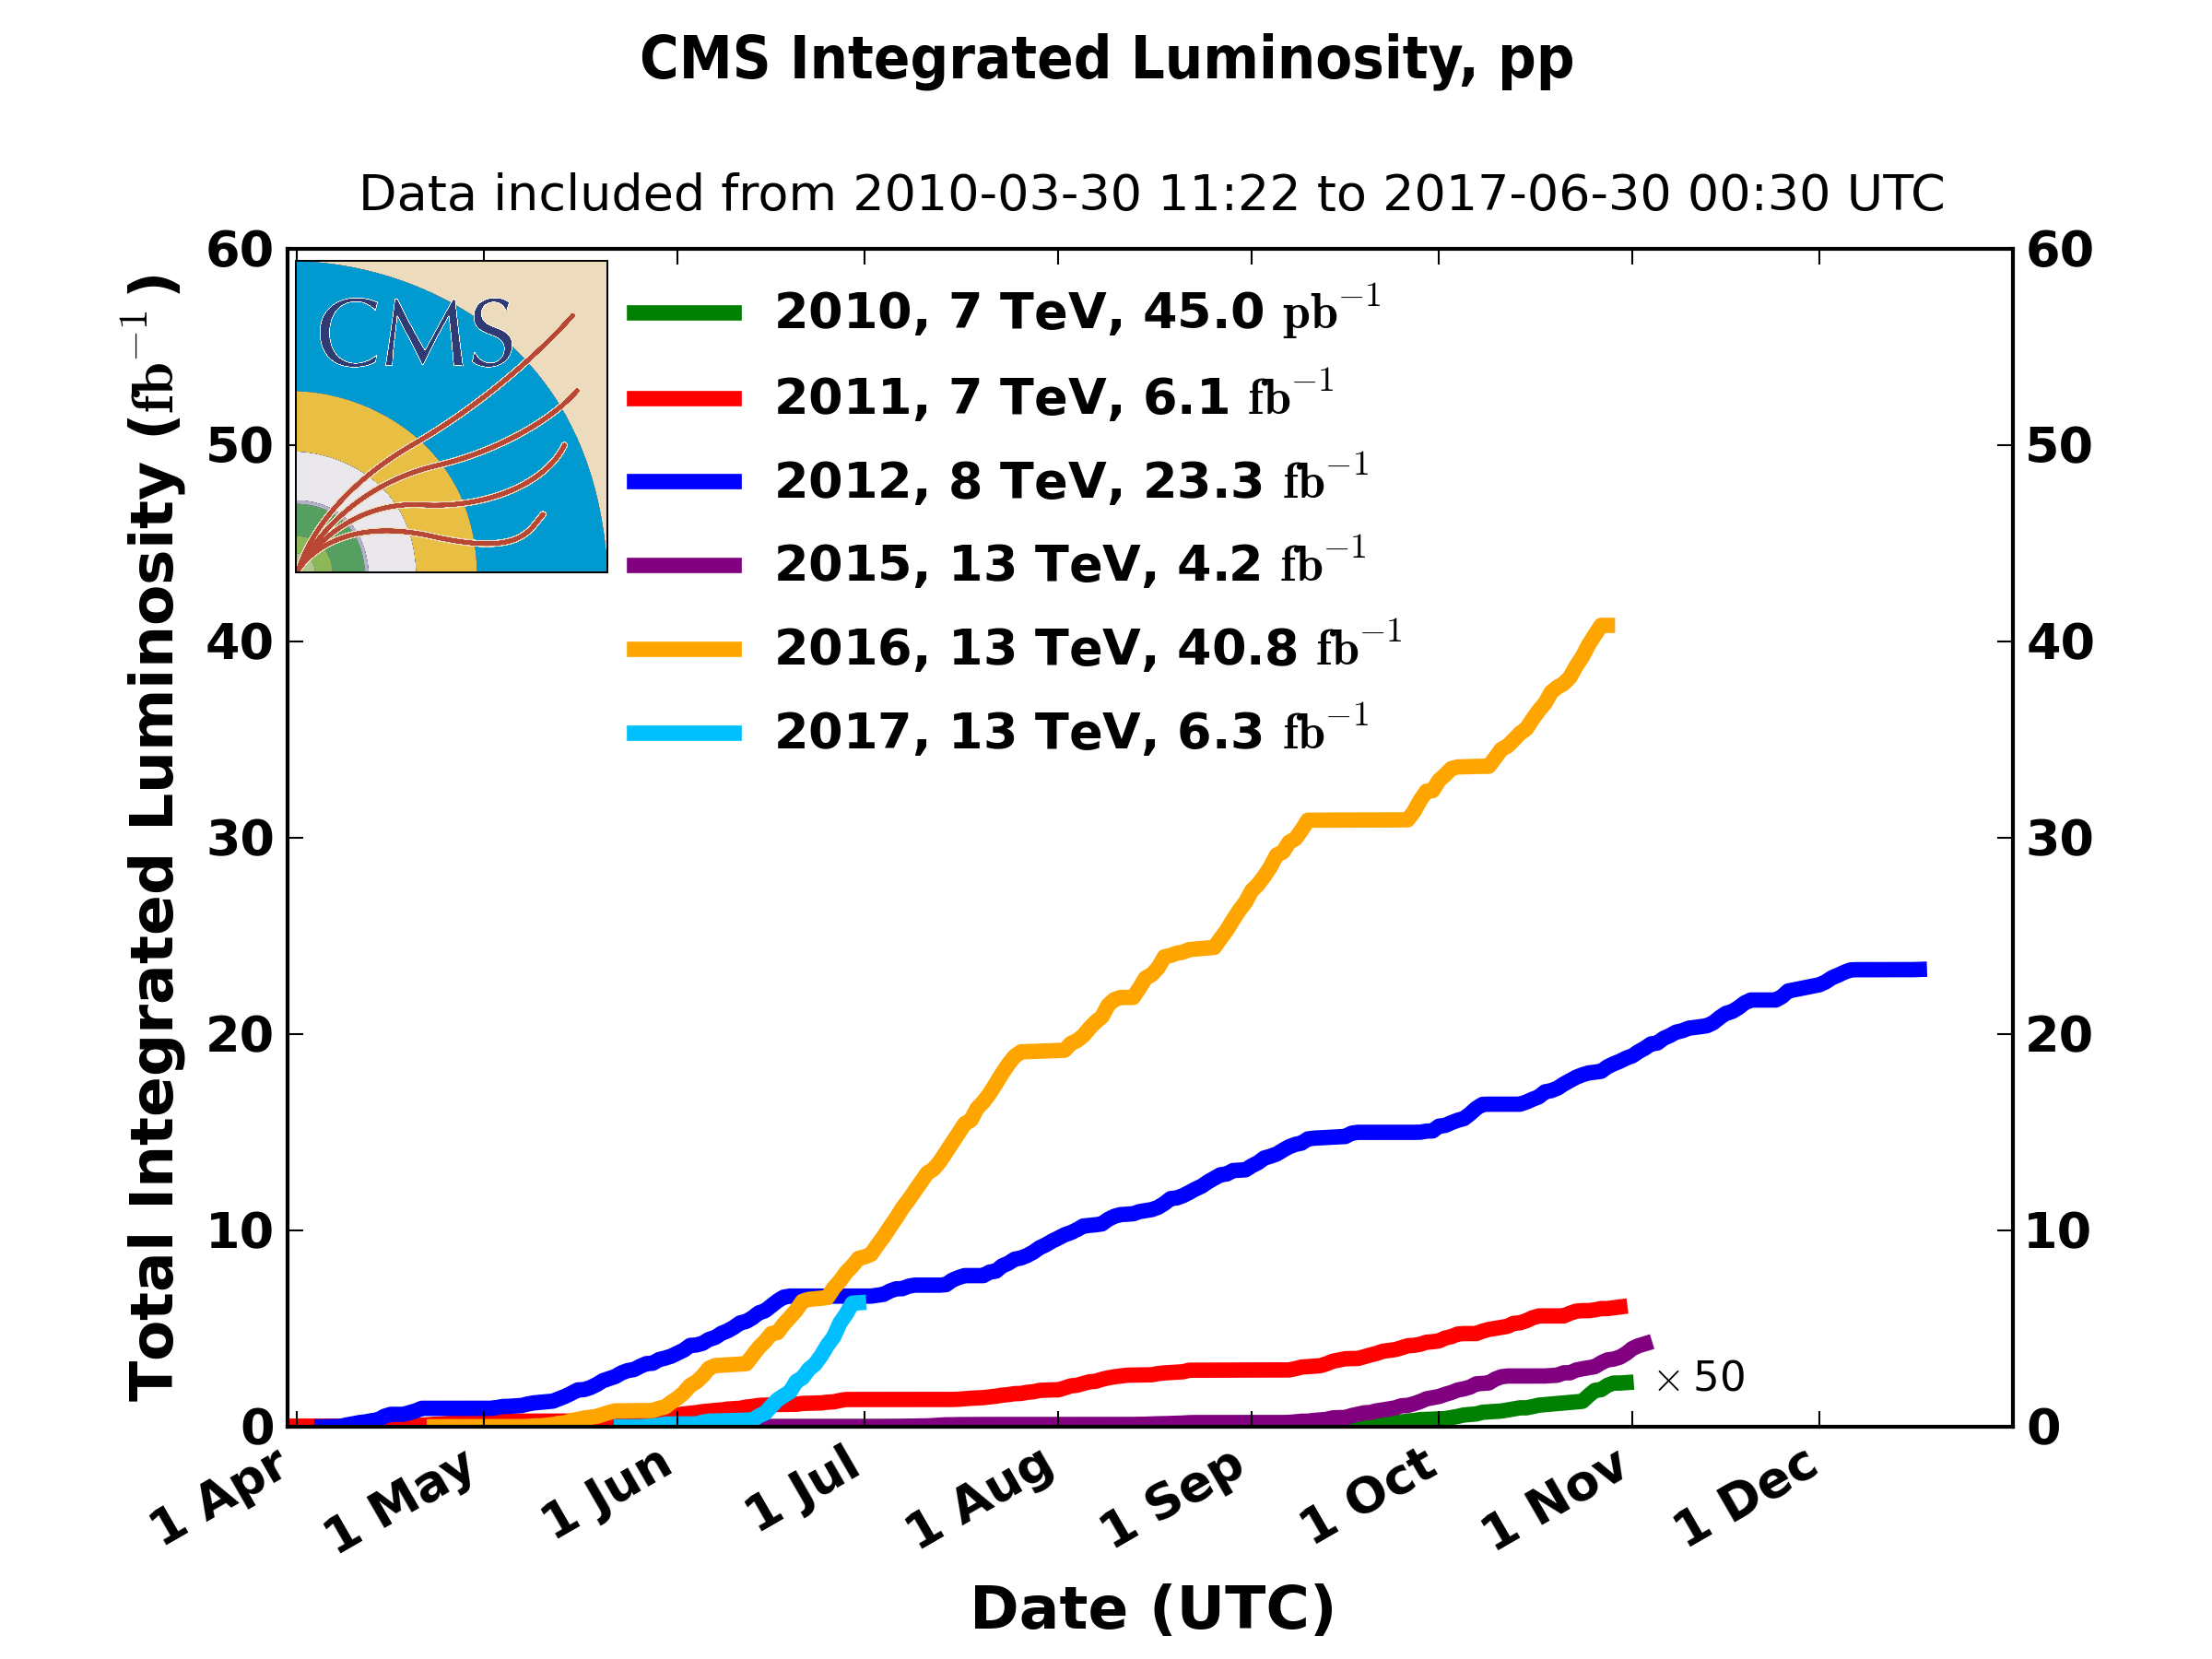
\includegraphics[width=.75\textwidth]{CMS_lumi_allyears}
 \caption{Overview of the integrated luminosity delivered to the CMS detector during Run~1 (2010 to 2012) and Run 2 (2015 to 2017).}
 \label{fig:lumi}
\end{figure}

\subsection{The experiments at the LHC}

There are four \acp{IP} where the proton or lead ion beams of the \ac{LHC} can collide, and around each of these points large particle detectors were built in order to record the generated collisions. The \acs{ATLAS} and \ac{CMS} detectors, located at \ac{IP}1 and \ac{IP}5, are both high luminosity general-purpose detectors and are consist of several layers surrounding the \ac{IP} in an onion-like structure to avoid particles escaping detection. These detectors can cover a wide range of high energy physics, from precision measurements of the Standard Model to searches beyond the Standard Model. At \ac{IP}2 the \acs{ALICE} detector is specialized in heavy ion collisions with low instantaneous luminosities, around $10^{27}$cm$^{-2}$s$^{-1}$. With this detector information is gathered about the quark-gluon plasma, a state of matter that exists at extremely high temperatures and densities where quarks and gluons are no longer confined in hadrons. The fourth main detector, \acs{LHCb}, is located at \ac{IP}8 and requires medium instantaneous luminosities of the order of a few $10^{32}$cm$^{-2}$s$^{-1}$. Using this detector $b$ quarks are being studied, focusing among other things on the matter-antimatter asymmetry.

\section{The CMS detector} 
\label{sec:CMS}

The searches described in this thesis were conducted using data collected with the \ac{CMS} detector, a general-purpose detector located on the \ac{LHC} ring. It consists of the typical components of a particle physics detector, namely a tracker, an \ac{ECAL}, a \ac{HCAL}, a solenoidal magnet, and muon detectors. One peculiar aspect is however that both calorimeters are situated inside the superconducting magnet. This design was chosen in order to improve the energy resolution by reducing the amount of material in front of the calorimeters. The detector has a length of 21.6 m, a diameter of 14.6 m and a total weight of 12500 t. A schematic overview is shown in Figure~\ref{fig:CMS}.

\begin{figure}[ht]
  \centering
 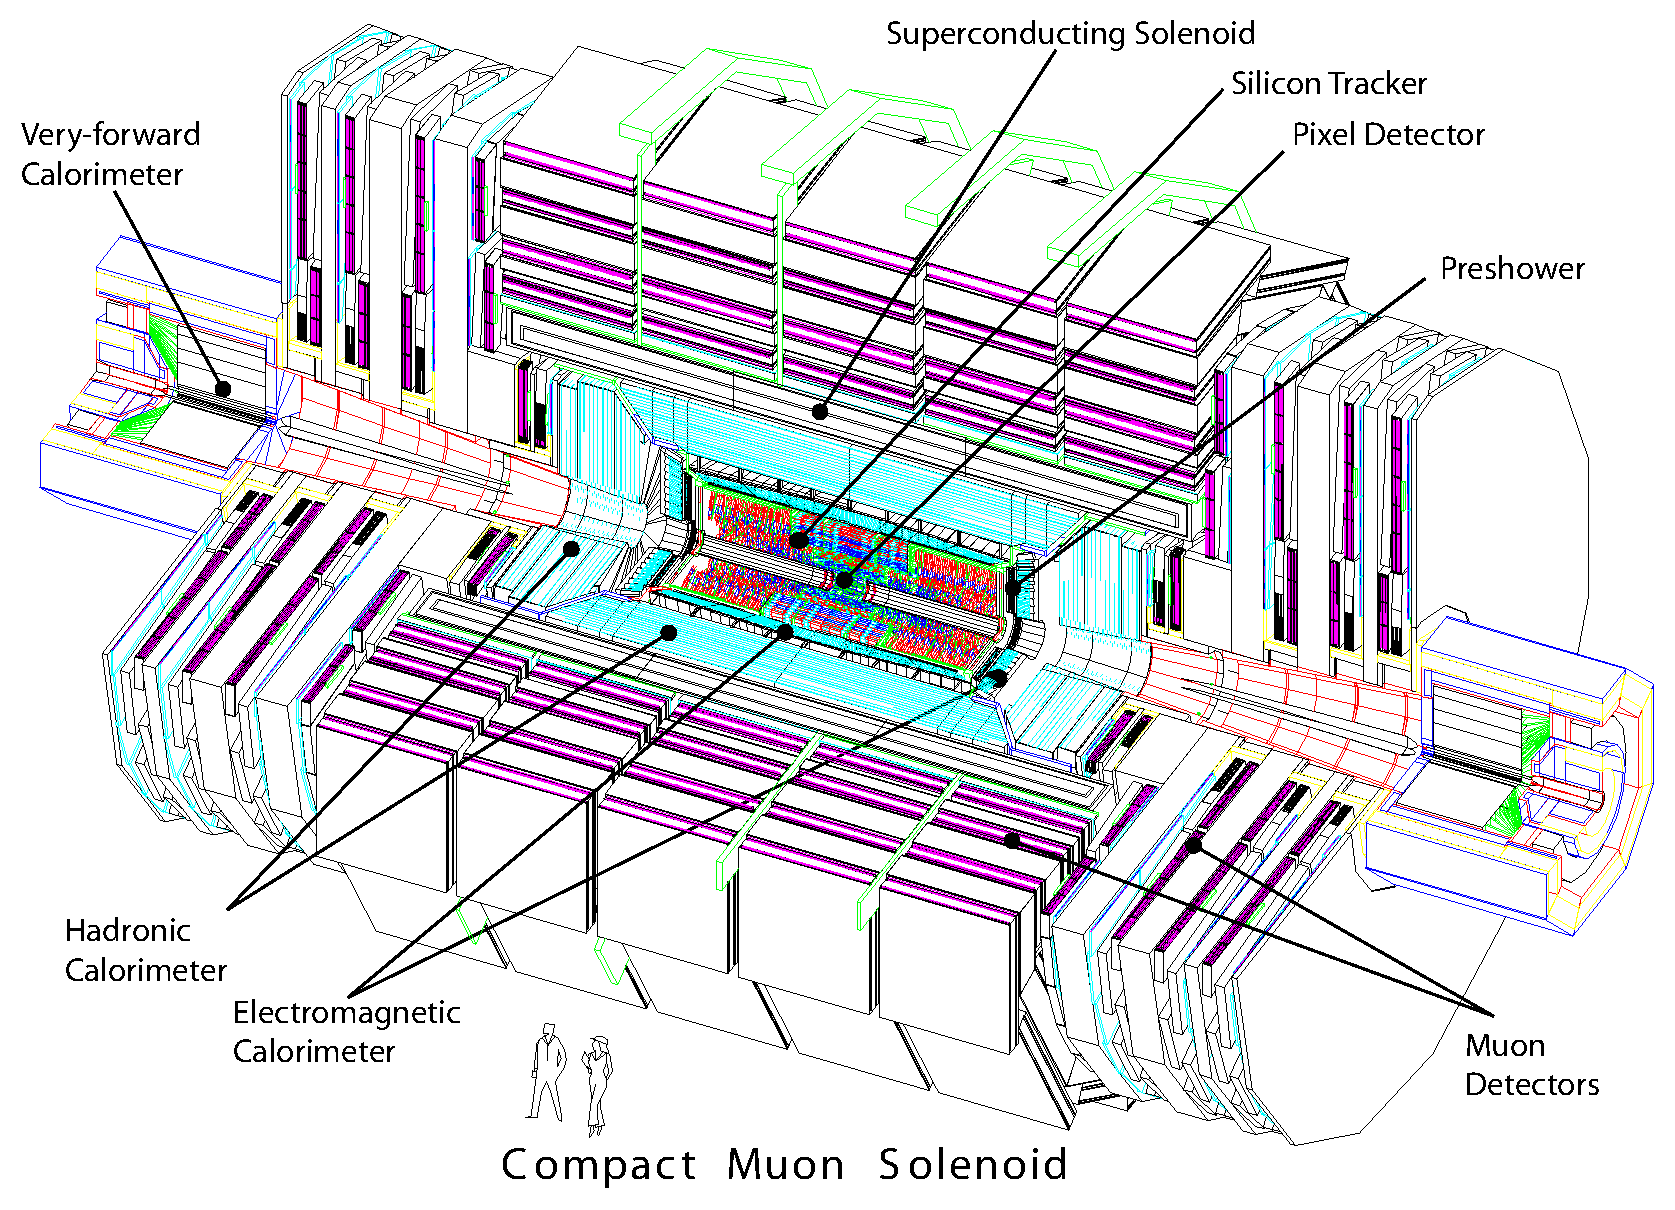
\includegraphics[width=.9\textwidth]{cms_complete_labelled}
 \caption{The \ac{CMS} detector, consisting of the pixel and strip tracker, the \protect\acf{ECAL} with preshower, the \protect\acf{HCAL} with its forward component, and the muon systems.}
 \label{fig:CMS}
\end{figure}

The CMS coordinate system places the origin at the nominal collision point. The $x$ axis is perpendicular to the beam and points towards the center of the \ac{LHC} ring, the $y$ axis is vertical and pointing upwards, and the $z$ axis is defined anti-clockwise along the beam direction. The azimuthal angle $\phi$ is then defined in the $xy$ plane, relative the the $x$ axis and the polar angle $\theta$ is measured with respect to the $z$ axis. In general, the polar angle is converted into the pseudorapidity
\begin{equation}
 \eta = -\ln\left(\tan\frac{\theta}{2}\right)
\end{equation}
for convenience, since differences in pseudorapidity are invariant under Lorentz boosts along the $z$ axis. A pseudorapidity of 0 corresponds to the direction perpendicular to the beam ($\theta = \pi/2$), and an infinite pseudorapidity corresponds to the direction parallel to the beam ($\theta = 0$).

Due to the conservation of momentum before and after the collision, the momenta of the particles in the final state of a collision should be balanced in the transverse plane. Another variable that is therefore often used in particle physics is the transverse momentum of a particle, defined as 
%the momentum component in the $xy$ plane:
\begin{equation}
p_T = p \cdot \sin \theta .
\end{equation}

\subsection{The tracker}

The innermost part of the \ac{CMS} detector, closest to the \ac{IP}, is the tracking system, which is designed to provide a precise measurement of the trajectory of charged particles. This all-silicon detector is divided into a pixel and a strip detector, with a layout as shown in Figure~\ref{fig:cmstracker}. The inner part, consisting of pixel modules, provides very precise 3D hits, which are important for vertex reconstruction and track seeding. This allows to have a precise measurement of secondary vertices and track impact parameters, necessary for the efficient identification of e.g. heavy flavor particles. As the hit occupancy is lower in the outer part of the detector, a larger cell size can be afforded, and silicon strips are used instead of pixels. This strip detector provides a large level arm and a link to the calorimeters and the muon system. The tracker covers a pseudorapidity range $|\eta| < 2.5$.

\begin{figure}[ht]
  \centering
 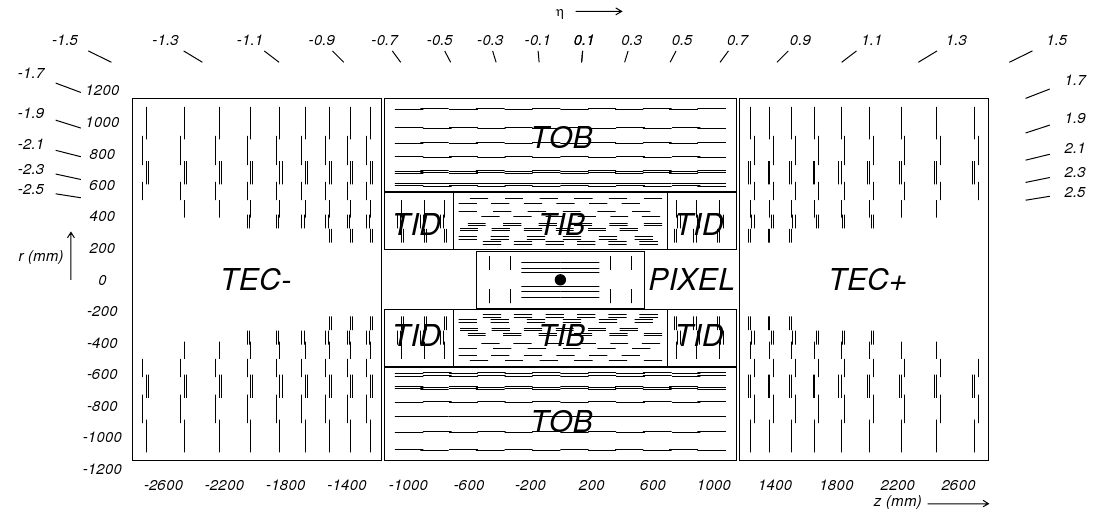
\includegraphics[width=.9\textwidth]{fig_cmstracker}
 \caption{A transverse view of the pixel and strip tracker detectors.}
 \label{fig:cmstracker}
\end{figure}

\subsubsection{The pixel tracker} 

The pixel tracker described here is the Phase 0 detector which was used to record the data used in this thesis, present for data-taking until 2016. During the extended technical stop in 2016 and 2017, it was replaced as a part of the \ac{CMS} Phase 1 upgrades. 

For the pixel modules n+ pixels on n-substrate are used, allowing the sensors to also work in under-depletion after type inversion. The 1440 modules are arranged in several cylindrical layers and disks, as illustrated in Figure~\ref{fig:cmstracker}. The barrel, consisting of 3 pixel layers surrounding the beam pipe at radii of 4.4, 7.3 and 10.2~cm, is complemented by the forward pixel detector, composed of 2 endcap disks on each side extending from 6 to 15~cm in radius. The barrel and the forward parts contain respectively 48 million and 18 million pixels with a size of $100 \times 150\ \mu\mathrm{m}^2$, covering a total area of 1.06~m$^2$.

In the barrel, the magnetic field of CMS is perpendicular to the drift of the electrons to the collecting pixels, which results in a Lorentz drift. This drift leads to a spread of the charge over several pixels. Since the read-out of the modules is analog, an improved spatial resolution can therefore be achieved with charge interpolation. In the forward pixel detector the drift of the electrons would be parallel to the magnetic field so in order to profit from the Lorentz angle, the modules are tilted by 20\degree in a turbine-like arrangement, as can be seen in Figure~\ref{fig:pix}. A spatial resolution of 10 $\mu$m (30 $\mu$m) can be achieved in the local directions $x$ ($y$) of the module, respectively. In the barrel $x$ is the longitudinal direction perpendicular the the beam and $y$ is the longitudinal direction parallel to the beam. 
%The resolution will degrade with radiation damage, since the charge-sharing will be reduced by a decrease in depletion depth or an increase of bias voltage.

\begin{figure}[ht]
  \centering
 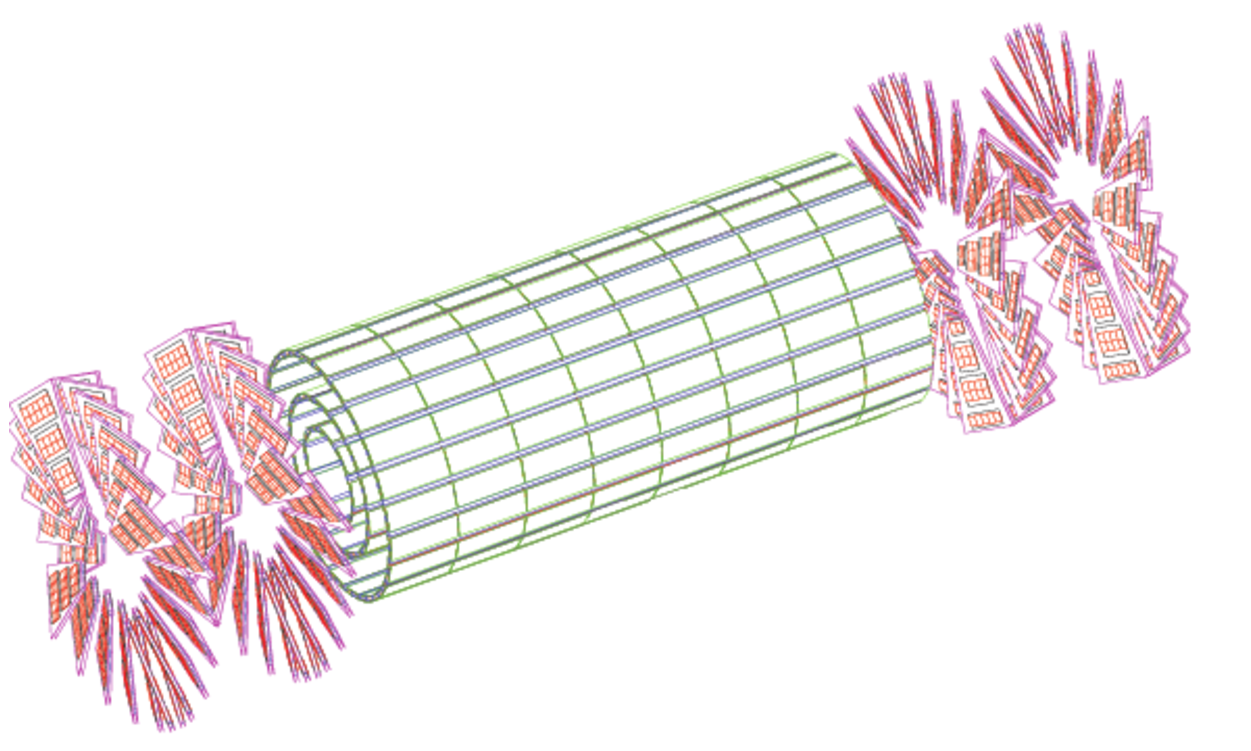
\includegraphics[width=.6\textwidth]{pixel}
 \caption{A 3D view of the barrel and forward pixel detector.}
 \label{fig:pix}
\end{figure}

The signals from the pixel sensors are read out by custom \acp{ROC}, which amplify and store the signals, and already apply zero-suppression on-detector. The data rate from the detector to the \acp{FED} is therefore not constant for every event. Additionally, if there are too many hits on a pixel module for a given event, they can not all be stored on the finite buffer of the \ac{ROC}. Consequently, as the instantaneous luminosity increases the pixel modules start to show a ``dynamic inefficiency''  which is most pronounced in the first layer, closest to the beampipe. This was one of the main motivations for the Phase 1 upgrade of the pixel detector.

\subsubsection{The strip tracker}

The outer part of the tracker consists of 15~148 strip modules, which are distributed among multiple barrel layers and endcap disks and make up a total active area of 198 m$^2$. The inner part is composed of 4 \ac{TIB} layers with 3 \ac{TID} on each side. Surrounding these are 6 \ac{TOB} layers and the 2 \ac{TEC}, which are composed of 9 disks. This geometric arrangement is shown in Figure~\ref{fig:cmstracker}, with double lines to indicate back-to-back modules. These so-called double-sided modules are mounted with a stereo angle of 100 mrad to improve the 3D point resolution by providing a measurement of the $z$ and $r$ co-ordinate in the barrel and disks, respectively.

In the \ac{TOB} and the 3 outermost rings of the \ac{TEC} two silicon sensors are daisy chained, while single sensors are used in the inner part. This is done to limit the number of read-out channels, since the area that had to be instrumented is larger in the outer region. The larger cell size can be afforded  due to the lower occupancy in the outer part. However, the noise of the sensors also increases with strip length, so thicker silicon sensors, 500 $\mu$m compared to 320$\mu$m in the inner part, are used in order to collect more signal per traversing particle.

The strip sensors are single sided p-on-n type silicon. The signals from the sensors are amplified, shaped, and stored by 4 or 6 custom APV25 chips per module. When the trigger has made a positive decision, the analog signals from two APV25 chips are multiplexed and sent to the \ac{FED} boards in the service cavern via optical fibers, where they are converted to digital signals. The \acp{FED} then perform pedestal and common mode subtraction as well as cluster finding. Additionally, the data is sparsified in these off-detector electronics, before being sent to the CMS central \ac{DAQ}. Due to charge sharing, this analog read-out scheme also results in an improved spatial resolution of 15 to 40 $\mu$m, depending on the position of the modules and the strip pitch. 

%Different strip pitch/width because

\subsubsection{Tracking}

The tracks of charged particles going through the \ac{CMS} tracker are reconstructed with an iterative tracking approach. This is used to cope with the high occupancy and consequently high combinatorics. Additionally, the first iterations search for tracks with less possible combinations, such as tracks with many pixel hits or a high momentum. After every iteration, the hits associated with the found track are removed to reduce the combinatorics. Each iteration consists of four steps:
\begin{enumerate}
 \item \textbf{Seed generation.} In this first step hits are combined into seeds for the subsequent track finding. In the initial iterations pixel triplets are used, then pixel pairs, in order to take gaps or non-working modules into account. Next, mixed pixel/strip triplets are taken, and finally strip-only seeds are used. These additional iterations improve the acceptance in $p_T$ and in displacement with respect to the primary vertex.
 \item \textbf{Track finding}. The seeds are used as starting point for a Kalman filter algorithm. This method extrapolates the seed trajectory outward to the next layer, taking into account potential energy loss and multiple scattering. If compatible hits are found in the next layer, the parameters of the trajectory are updated. This process continues until the outermost layer of the tracking system. Using this method, a given seed can generate multiple tracks, or different tracks can share hits. A trajectory cleaner therefore determines the fraction of hits the tracks have in common and discards the track with the lowest number of hits when there are too many shared hits. If both tracks have the same number of hits, the track with the largest $\chi^2$ value is removed.
 \item \textbf{Track fitting.} The track parameters are then refitted using a Kalman filter and smoother, taking all hits determined in the track finding step into account.
 \item \textbf{Track selection.} Finally, the tracks are selected based on quality requirements, such as the number of layers that have hits, the $\chi^2/$dof, and the distance to a primary vertex. This greatly reduces the fraction of reconstructed tracks that are fake.
\end{enumerate}

The performance of the track reconstruction is excellent, and a high track-finding efficiency is obtained~\cite{Chatrchyan:2014fea} while keeping the rate of fake tracks negligible. The highest tracking efficiency is obtained for muons, which traverse the full detector volume and have an improved momentum resolution due to tracking information from the muon detectors giving a long lever arm. For isolated muons with $p_T$ between 1 and \SI{100}{GeV} the tracking efficiency is higher than 99\% for the entire $\eta$ coverage of the tracker, as can be seen from the left plot in Figure~\ref{fig:eff_eta}. The $p_T$ resolution is about 2-3\% for a muon with $p_T = $ \SI{100}{GeV} up to $|\eta| < 1.6$, but worsens for higher pseudorapidities. Different types of particles interact differently with the detector material. Charged hadrons, for example, are also subject to elastic and inelastic nuclear interactions and have a tracking efficiency of 80-95\% depending on pseudorapidity and transverse momentum, as shown in the right plot of Figure~\ref{fig:eff_eta}.

\begin{figure}[ht]
  \centering
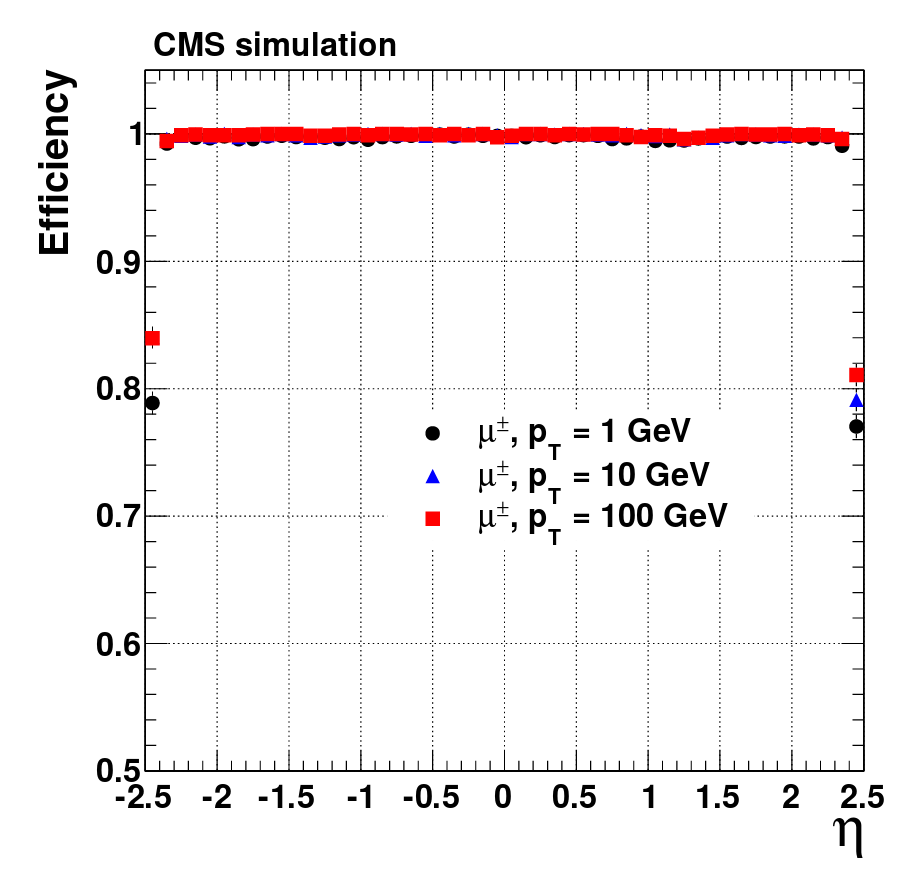
\includegraphics[width=.4\textwidth]{muon_eff_eta}\hspace{1cm}
 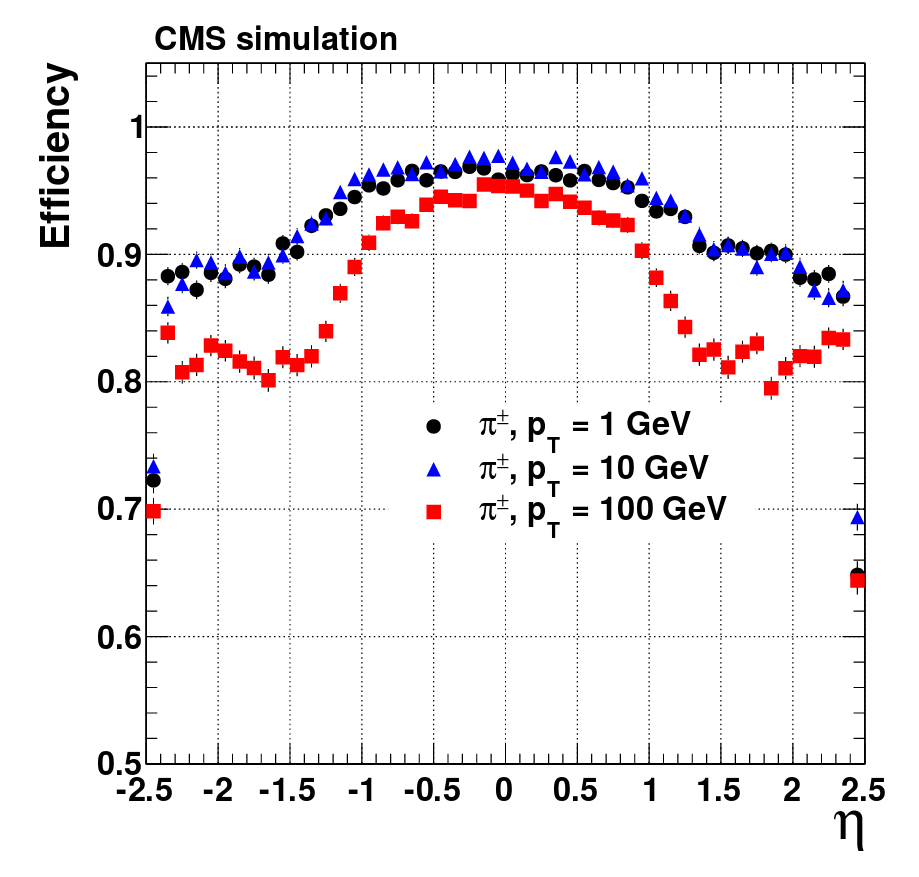
\includegraphics[width=.4\textwidth]{pion_eff_eta} 
 \caption{The muon efficiency (left) and pion efficiency (right) as a function of pseudorapidity, for multiple transverse momenta.~\cite{Chatrchyan:2014fea}}
 \label{fig:eff_eta}
\end{figure}

Finally, the primary vertex is reconstructed from the tracks. Since the collisions happen between bunches of protons, multiple protons will be colliding at the same time. The extra collisions, next to the potentially interesting collision, are referred to as pile-up interactions. The particles generated in these collisions are all detected simultaneously and form a challenge to disentangle them from the particles coming from the to be studied interaction.

The reconstruction is done in 2 steps: first the tracks that appear to originate from the same interaction vertex are clustered, then a fitting procedure computes the vertex parameters and assigns a weight to each associated track, reflecting the probability that it corresponds to the considered vertex. Figure~\ref{fig:PV} shows the reconstruction efficiency and the resolution of the primary vertex. The more tracks, the better the vertex is constrained and thus the better the resolution.

\begin{figure}[ht]
  \centering
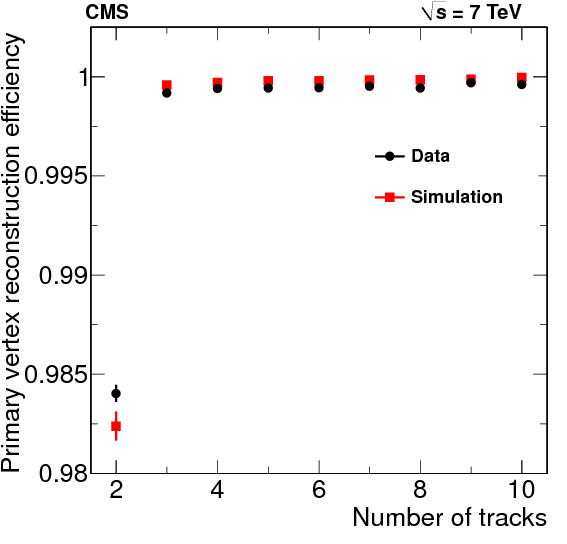
\includegraphics[width=.4\textwidth]{PV_eff}\hspace{1cm}
 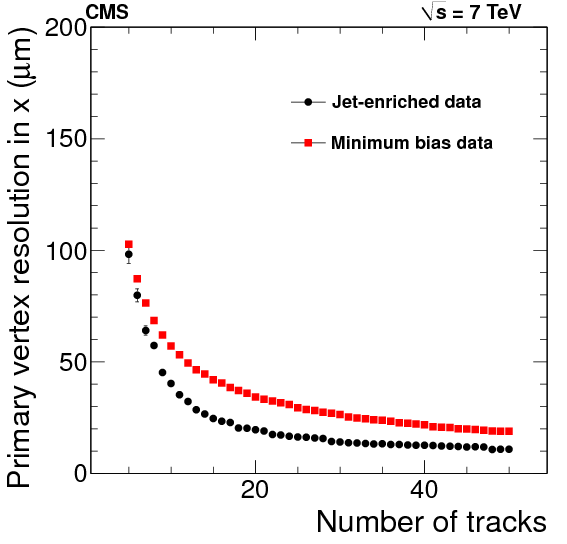
\includegraphics[width=.4\textwidth]{PV_res} 
 \caption{The primary vertex reconstruction efficiency (left) and resolution (right) as a function of the number of tracks associated to it.~\cite{Chatrchyan:2014fea}}
 \label{fig:PV}
\end{figure}

\subsection{The electromagnetic calorimeter}

Surrounding the tracker, the \ac{CMS} \acf{ECAL} is designed to measure the energy of photons and electrons. It is composed of 75~848~lead tungstate (PbWO$_4$) crystals arranged in a cylindrical barrel and 2 endcaps. The barrel crystals measure $22\times22\, \mathrm{mm}^2$ at the front face of crystal, and $26\times26\, \mathrm{mm}^2$ at the rear face, which corresponds to approximately $0.0174\times0.0174$ in $\eta$-$\phi$. The length of the crystal is \SI{230}{mm}, corresponding to $25.8$ radiation lengths. In the endcaps, the crystals have a rear face cross section of $30\times30\, \mathrm{mm}^2$, front face cross section of $28.62\times28.62\, \mathrm{mm}^2$, and a length of \SI{220}{mm}, corresponding to 24.7 radiation lengths. 

The high density material was chosen due to its short radiation length and small Moli\'ere radius, resulting in a small spread of the electromagnetic shower generated by an incoming photon or electron. This allows for a fine granularity, a better shower separation, and a compact calorimeter. Additionally, this scintillating material has a fast response, as about 80\% of the light is emitted during the first \SI{25}{ns}. The scintillation light is collected by photodetectors, digitized, and read out.

The layout of the \ac{ECAL} is shown in Figure~\ref{fig:ecal}, with the barrel (EB) extending up to $|\eta| < 1.470$ and the endcaps (EE) on each side covering the range $1.479 < |\eta| < 3.0$. A preshower detector (ES) is positioned in front of the endcap crystals, covering the pseudorapidity range between $|\eta|=1.653$ and $|\eta| = 2.6$. This detector consists of a layer of lead which initiates an electromagnetic shower from incoming photons or electrons, and a layer of silicon sensors which measures the deposited energy. The main goal of this 20~cm thick detector is to discriminate between photons and neutral pions.

\begin{figure}[ht]
 \centering
 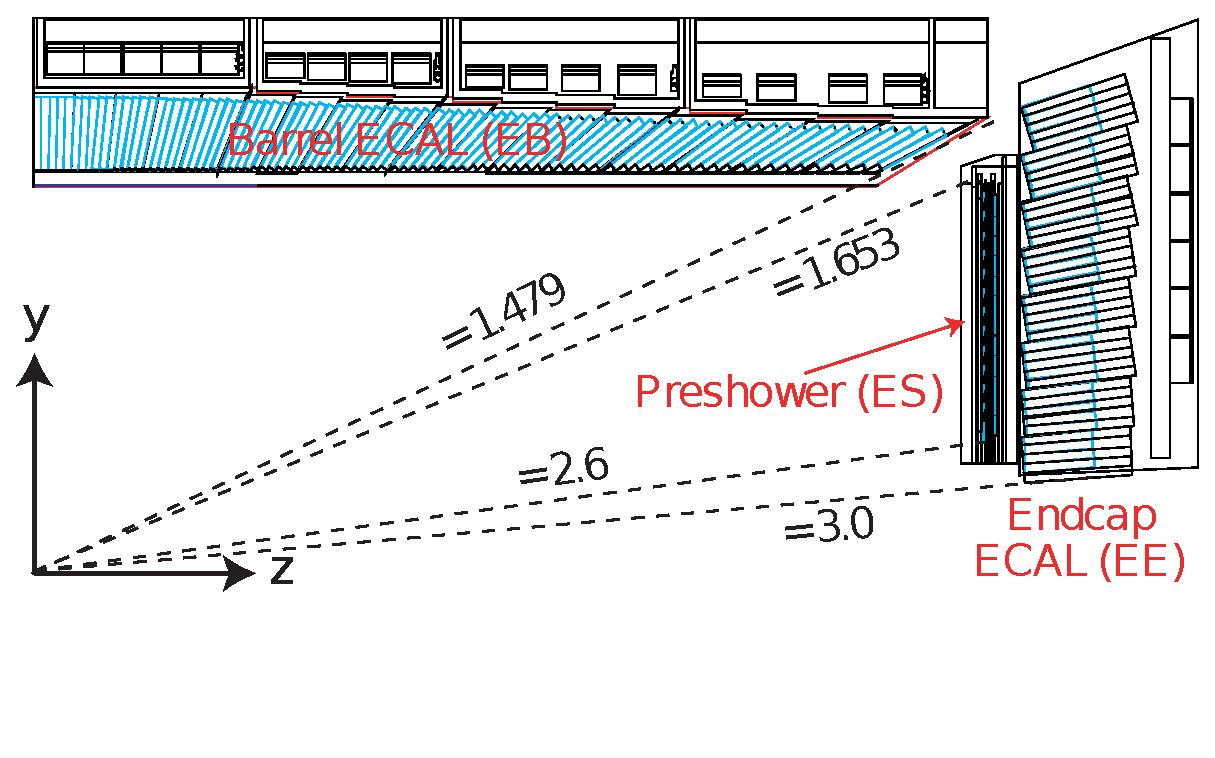
\includegraphics[width = .8\textwidth]{Transverse_section}
\caption{A transverse view parallel to the beamline showing one quarter of the \ac{ECAL}, with its barrel (EB), endcap (EE), and preshower (ES) detectors.}
\label{fig:ecal}
\end{figure}

The energy resolution of calorimeters can be parametrized by the following stochastic ($S$), noise ($N$), and constant ($C$) terms:
\begin{equation}
\label{eq:energy_resolution}
 \left(\frac{\sigma}{E}\right)^2 = \left(\frac{S}{\sqrt{E}}\right)^2 + \left(\frac{N}E{}\right)^2 + C^2
\end{equation}
The stochastic term represents contributions from the shower containment, the number of photoelectrons and the fluctuations in the gain process.  The noise term takes into account all noise components, such as electronics and digitization noise. Finally, the constant term characterizes among others energy leakage from the back of the calorimeter crystals and non-uniformities of the longitudinal light collection. The latter term dominates the energy resolution for high-energy electron and photon showers. Figure~\ref{fig:ecal_res} shows the energy dependence of this resolution for incident electrons as measured in a beam test, as well as the determined stochastic, noise, and constant terms obtained by fitting  equation~\ref{eq:energy_resolution} to the data.

\begin{figure}[ht]
 \centering
 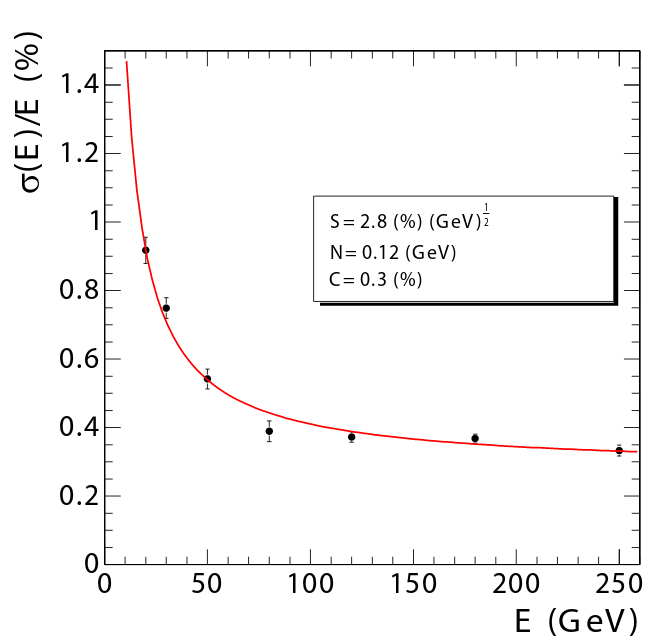
\includegraphics[width = .6\textwidth]{ecal_res}
\caption{The \ac{ECAL} energy resolution as a function of the electron energy, measured from a beam test. The stochastic ($S$), noise ($N$), and constant ($C$) are given as well.}
\label{fig:ecal_res}
\end{figure}

A more recent measurement of the energy resolution was performed using electrons from Z boson decays in collision data. In the central region, up to $|\eta| < 0.8$, it was measured to be better than 2\%. Outside of this region, in the more forward direction, the energy resolution is 2-5\%~\cite{Chatrchyan:2013dga}. The reconstruction of the electrons and photons will be discussed in Section~\ref{sec:electron_reconstruction}.

\subsection{The hadronic calorimeter}

The \acf{HCAL} surrounds the \ac{ECAL} with the aim to measure the energy of charged and neutral hadrons. The missing transverse energy can then be inferred from this measurement together with the measured energy in the \ac{ECAL}, in order to identify neutrinos or exotic particles. The \ac{HCAL} consists of brass absorber plates interleaved with plastic scintillator tiles.

Figure~\ref{fig:hcal} shows a longitudinal quarter view of the different \ac{HCAL} components. A cylindrical barrel (HB) covers the region up to $|\eta| < 1.4$ and is complemented by endcaps (HE) on each side, extending the pseudorapidity range to $|\eta| < 3.0$. In the central region, the stopping power of the \ac{ECAL} and \ac{HCAL} barrel is not sufficient to contain the entire hadron showers. The \ac{HCAL} was therefore extended outside the solenoid with an outer calorimeter (HO), which uses the the magnet coil as absorber and consists of scintillators. Two layers are positioned at $\eta = 0$, where the absorber depth is minimal, and only 1 layer is used for the 2 rings on each side of the central ring. Finally, a forward calorimeter (HF) is positioned at 11.2~m from the \ac{IP} covering $3.0 < |\eta| < 5.2$. Unlike the other \ac{HCAL} components, this detector consists of iron and quartz fibers. Cherenkov-based, radiation-hard technology, since it is exposed to very large particle fluxes. 
% Additionally, the forward detector is used as luminosity monitor.

\begin{figure}[ht]
  \centering
 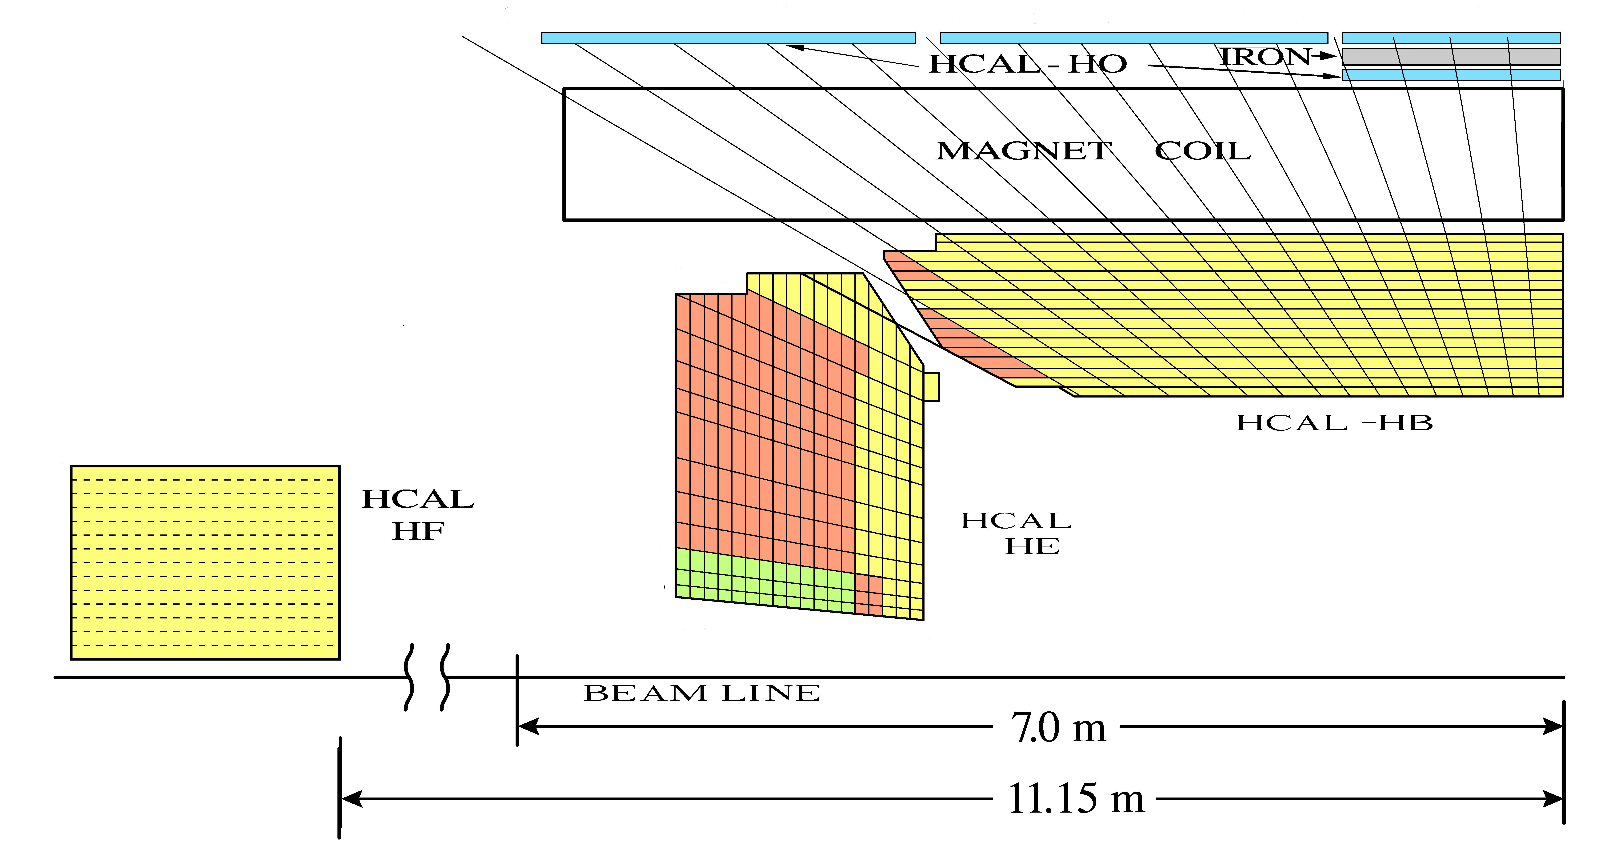
\includegraphics[width=.8\textwidth]{hcal}
 \caption{A quarter view of the \protect\acf{HCAL}, parallel to the beamline. The barrel (HB), endcap (HE), outer (HO), and forward (HF) detectors are indicated.}
 \label{fig:hcal}
\end{figure}

The optical signals from the scintillators in the HB and HE are converted to electrical signals by multichannel hybrid photodiodes, while silicon photomultipliers (SiPMs) are used in the HO. In the HF, the Cherenkov light emitted in the quartz fibers is detected by standard photomultiplier tubes (PMTs), since the magnetic field is much smaller in this region.

The expected transverse energy resolution for jets is shown in Figure~\ref{fig:JER} for various pseudorapidity regions: barrel jets ($|\eta| < 1.4$), endcap jets ($1.4 < |\eta| < 3.0$), and very forward jets ($3.0 < |\eta| < 5.0$). Details about the reconstruction of jets from calorimeter and tracking information will be given in Section~\ref{sec:jet_reconstruction}.

\begin{figure}[ht]
  \centering
 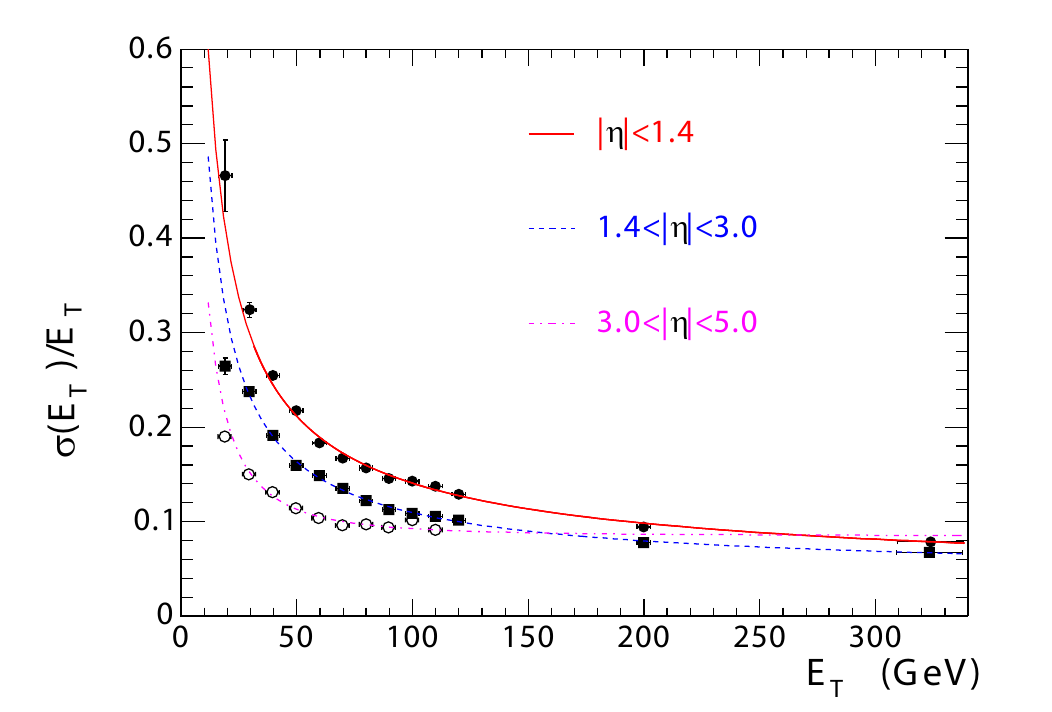
\includegraphics[width=.6\textwidth]{JER}
 \caption{The jet transverse energy resolution as a function of the jet transverse energy, for barrel jets ($|\eta| < 1.4$), endcap jets ($1.4 < |\eta| < 3.0$), and very forward jets ($3.0 < |\eta| < 5.0$).}
 \label{fig:JER}
\end{figure}

\subsection{The muon system}

The outermost detector, located entirely on the outside of the solenoid, is a dedicated muon detection system. The purpose of this subsystem is muon identification, momentum measurement, and triggering. As illustrated in Figure~\ref{fig:muons}, the layers of muon chambers are embedded in the iron yoke constraining the magnetic field lines. The strong magnetic field completely saturates the return yoke with a field of about \SI{2}{T}, in opposite direction with respect to the field inside the magnet.

Three different types of gaseous detectors are used. In the barrel, 4 layers of \ac{DT} are installed, covering the pseudorapidity range up to $|\eta| < 1.2$. Due the higher flux and the larger and non-uniform magnetic field at larger pseudorapidities, \ac{CSC} are used in the endcap region ($0.9 < |\eta| < 2.4$). The \acp{DT} are designed for the low muon rates that are expected in the barrel and thus have a slower response time than the \acp{CSC}. \acp{RPC} complement the \ac{DT} and \ac{CSC} systems in the pseudorapidity region up to $|\eta| < 1.8$. They provide a fast response, with a good time resolution but a worse spatial resolution than the \acp{DT} or \acp{CSC}. The \acp{RPC} are therefore very well suited to trigger on muons.

\begin{figure}[ht]
  \centering
 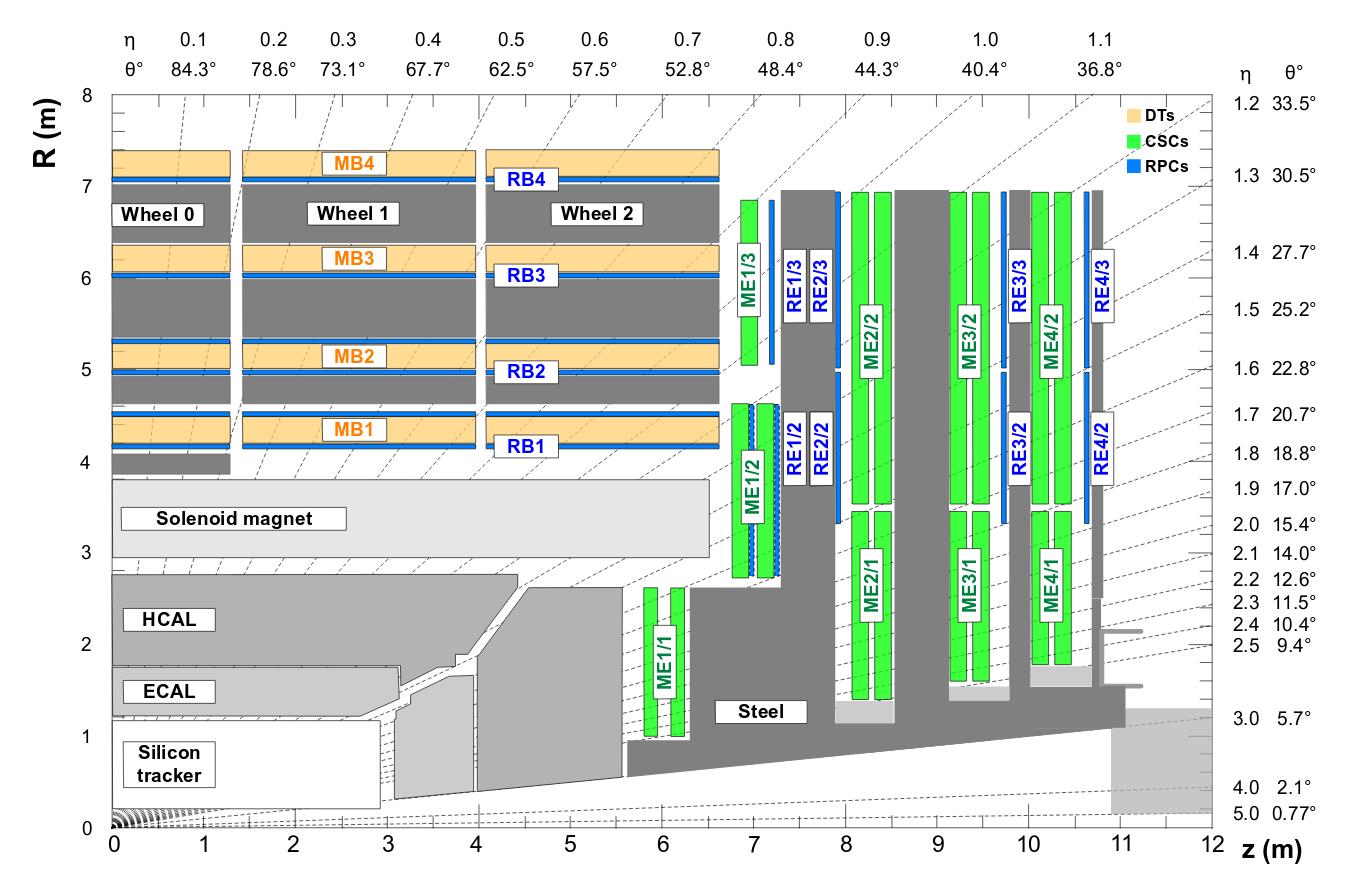
\includegraphics[width=.9\textwidth]{muon_system_new}
 \caption{A transverse view of one quarter of \ac{CMS} showing the position of the 3 types of muon detectors. The \protect\acf{DT} are located in the barrel, the \protect\acf{CSC} in the endcaps, and the \protect\acf{RPC} in both regions up to $|\eta| < 1.8$.}
 \label{fig:muons}
\end{figure}

The offline reconstruction efficiency of simulated events containing one muon is typically between 95\% and 99\%, except for the regions between 2 \ac{DT} wheels ($|\eta| = 0.25$ and $|\eta| = 0.8$) and the transition region between the \acp{DT} and \acp{CSC} ($|\eta| = 1.2$), where the efficiency drops to 92\%. The reconstruction of muons using the information from the tracker and the muon detectors will be detailed in Section~\ref{sec:muon_reconstruction}. For low pseudorapidities and small momenta, the offline momentum resolution of the standalone muon system is about 9\%. At momenta around \SI{1}{TeV}, the resolution varies from 15\% to 40\%, depending on the pseudorapidity. As demonstrated in Figure~\ref{fig:muon_res}, performing a global momentum fit using the tracker as well improves the resolution by an order of magnitude at low muon momenta. At high momenta the resolution of the full system is about 5\%.

\begin{figure}[ht]
  \centering
 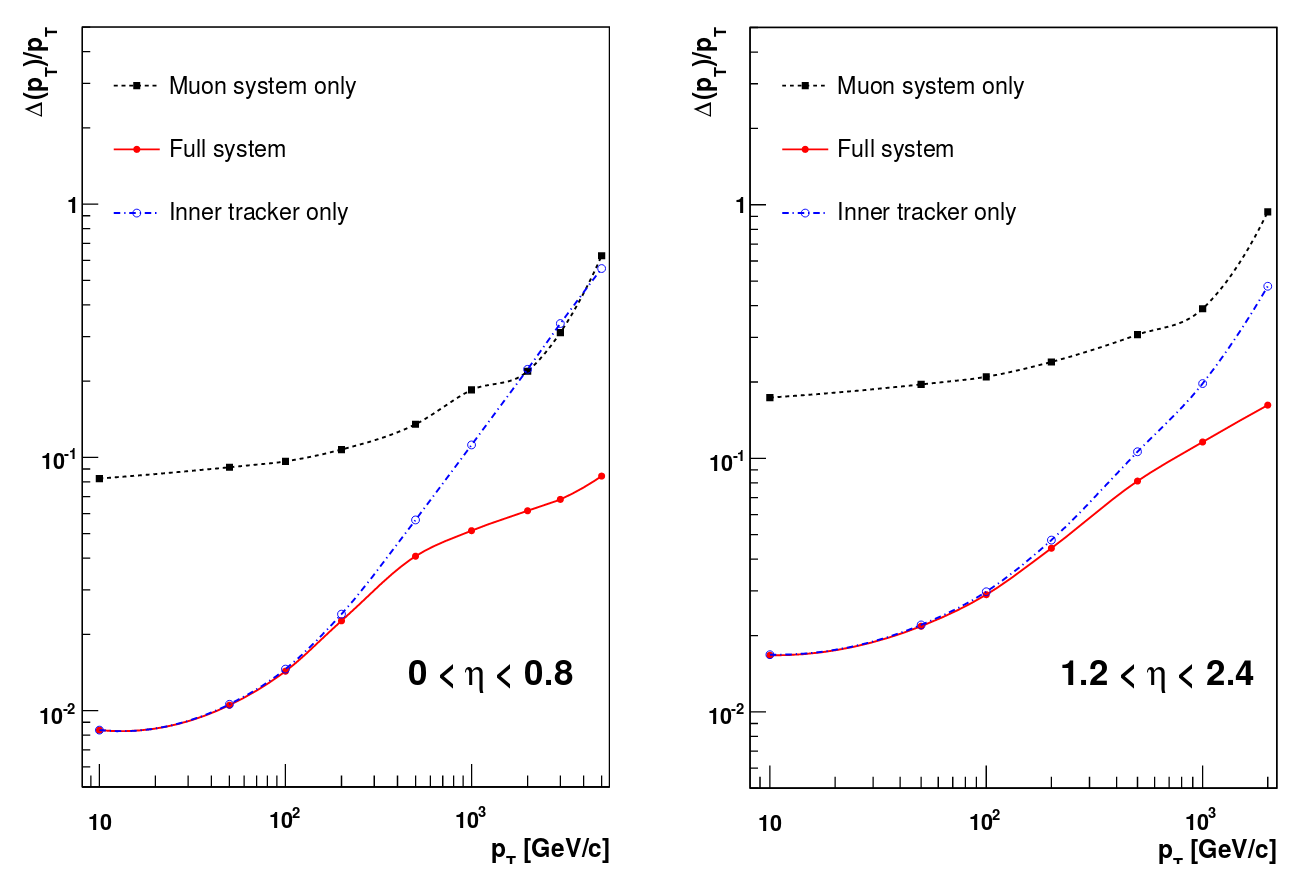
\includegraphics[width=.9\textwidth]{muon_res}
 \caption{The muon transverse momentum resolution as a function of transverse momentum for low (left) and (high) pseudorapidities. The resolution is shown for the muon system and the tracker separately, and for the full system.~\cite{Chatrchyan:2008aa}}
 \label{fig:muon_res}
\end{figure}

\subsection{Trigger and data acquisition}

Collisions are provided by the \ac{LHC} at high interaction rates, with an interval of \SI{25}{ns} between bunch crossings. This corresponds to a frequency of \SI{40}{MHz}. Additionally, multiple collisions occur at the same time, depending on the luminosity. Since it is impossible to store and process the large amount of data produced in the collisions at this high rate, a severe rate reduction is needed. This rate reduction is performed by the trigger system, which decides whether to store or reject an event. Since this decision process is constrained in time, the computing time is optimized by rejecting uninteresting events as quickly as possible. The rate is reduced to \SI{1}{kHz} in two steps by the \ac{L1} Trigger and the \ac{HLT}.

The \ac{L1} Trigger decision is based on information from the calorimeters and muon systems, following the structure illustrated in Figure~\ref{fig:L1}. At the lowest level, the Local Triggers are based on energy deposits in calorimeter towers and track segments or hit patterns in the muon system. Regional triggers, indicated as Calo Trigger Layer 1 and Muon Track-Finder Layer in the figure, then combine this information and use pattern logic to determine trigger objects such as jet or muon candidates in separated spatial regions. The candidates are ranked based on their energy or momentum and quality, reflecting the level of confidence assigned to the \ac{L1} parameter measurements. Finally, the Calo Trigger Layer 2 and the Global Muon Trigger~(GMT) determine the highest-rank calorimeter and muon objects across the whole detector and transfer them to the Global Trigger, which makes the final decision to accept or reject an event. Following this procedure, the \ac{L1} Trigger thresholds are tuned to reduce the event rate to 100~kHz. The \ac{L1} Trigger is composed of custom electronics located partially on the detectors, and partially in the underground service cavern. The \ac{L1} decision needs to be made and distributed to the detector front-end electronics within 3.8~$\mu$s~\cite{Tapper:2013yva}.

\begin{figure}[ht]
  \centering
 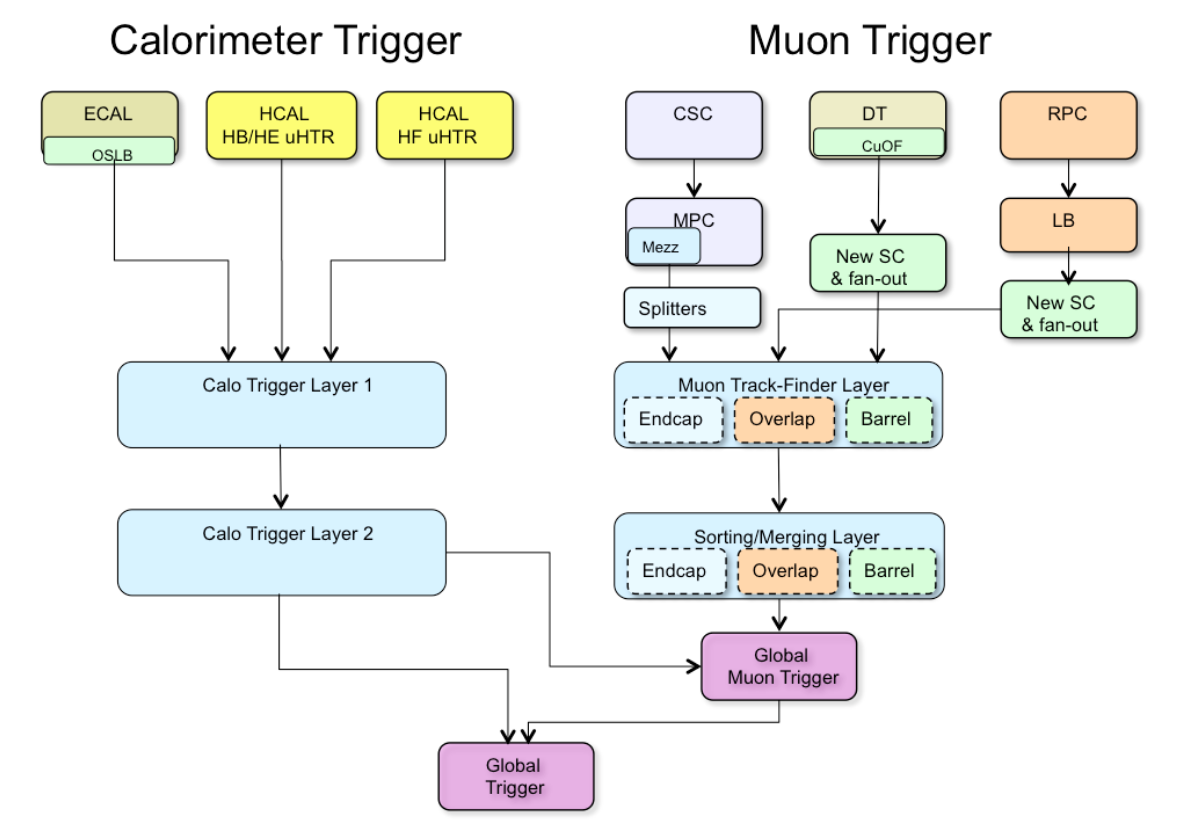
\includegraphics[width=.9\textwidth]{trigger}
 \caption{Schematic overview of the \ac{L1} Trigger.~\cite{Tapper:2013yva}}
 \label{fig:L1}
\end{figure}
 % figure from: http://cds.cern.ch/record/2238553/files/CR2016_412.pdf
 
The readout of the data proceeds as illustrated in Figure~\ref{fig:DAQ}. When an event is accepted by the \ac{L1} Trigger, the data from about $740$ \acp{FED} is read out by the \acp{RU}. For so-called {\it legacy} systems, i.e. systems which are using VME-based hardware from the initial installation, the \acp{FED} are read out by custom Front-End-Readout-Link (FRL) cards, while for systems that changed their readout architecture from the VME standard to the newer $\rm \mu{}$TCA standard during or after LS1 they are read out via the newer Front-End-Readout-Optical-Link (FEROL) cards. The event fragments are then sent over the event-builder switch to the \acp{BU}, which assemble the events. Next, the events are distributed to the \acp{FU} by a large switch network.

\begin{figure}[ht]
  \centering
 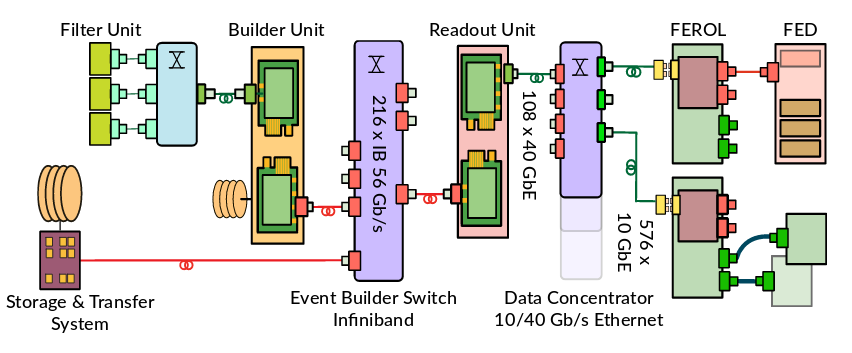
\includegraphics[width=.9\textwidth]{DAQ}
 \caption{Schematic of the \protect\acf{DAQ} system.~\cite{Andre:2252634}}
 \label{fig:DAQ}
\end{figure}

The \ac{HLT} software system is implemented in this filter farm, which uses more than 15000 CPU cores for the final event selection. In this second step, the \ac{HLT} reduces the event rate further to \SI{1}{kHz}. The complete read-out data, including information from the pixel and strip tracker, are available for this step. New objects can therefore be reconstructed such as e.g. tau leptons and b-jets, as is done in the offline software, but speed-optimized.%http://ieeexplore.ieee.org/stamp/stamp.jsp?arnumber=7111380

\subsection{CMS performance in Run 2}

The number of collisions recorded at the experiments will differ from the amount delivered by the \ac{LHC}. Data loss can be caused by e.g. problems with a particular subdetector, the trigger rate, the data acquisition, or the infrastructure. During Run 2, CMS achieved a data taking efficiency of 89\% and 92\% in 2015 and 2016, respectively. The comparison between the delivered and recorded cumulative integrated luminosity in 2016 is shown in Figure~\ref{fig:CMSlumi}. Subsequently, the recorded data is certified by the offline \ac{DQM}, to ensure that the data are suited for physics analysis. 

\begin{figure}[ht]
  \centering
 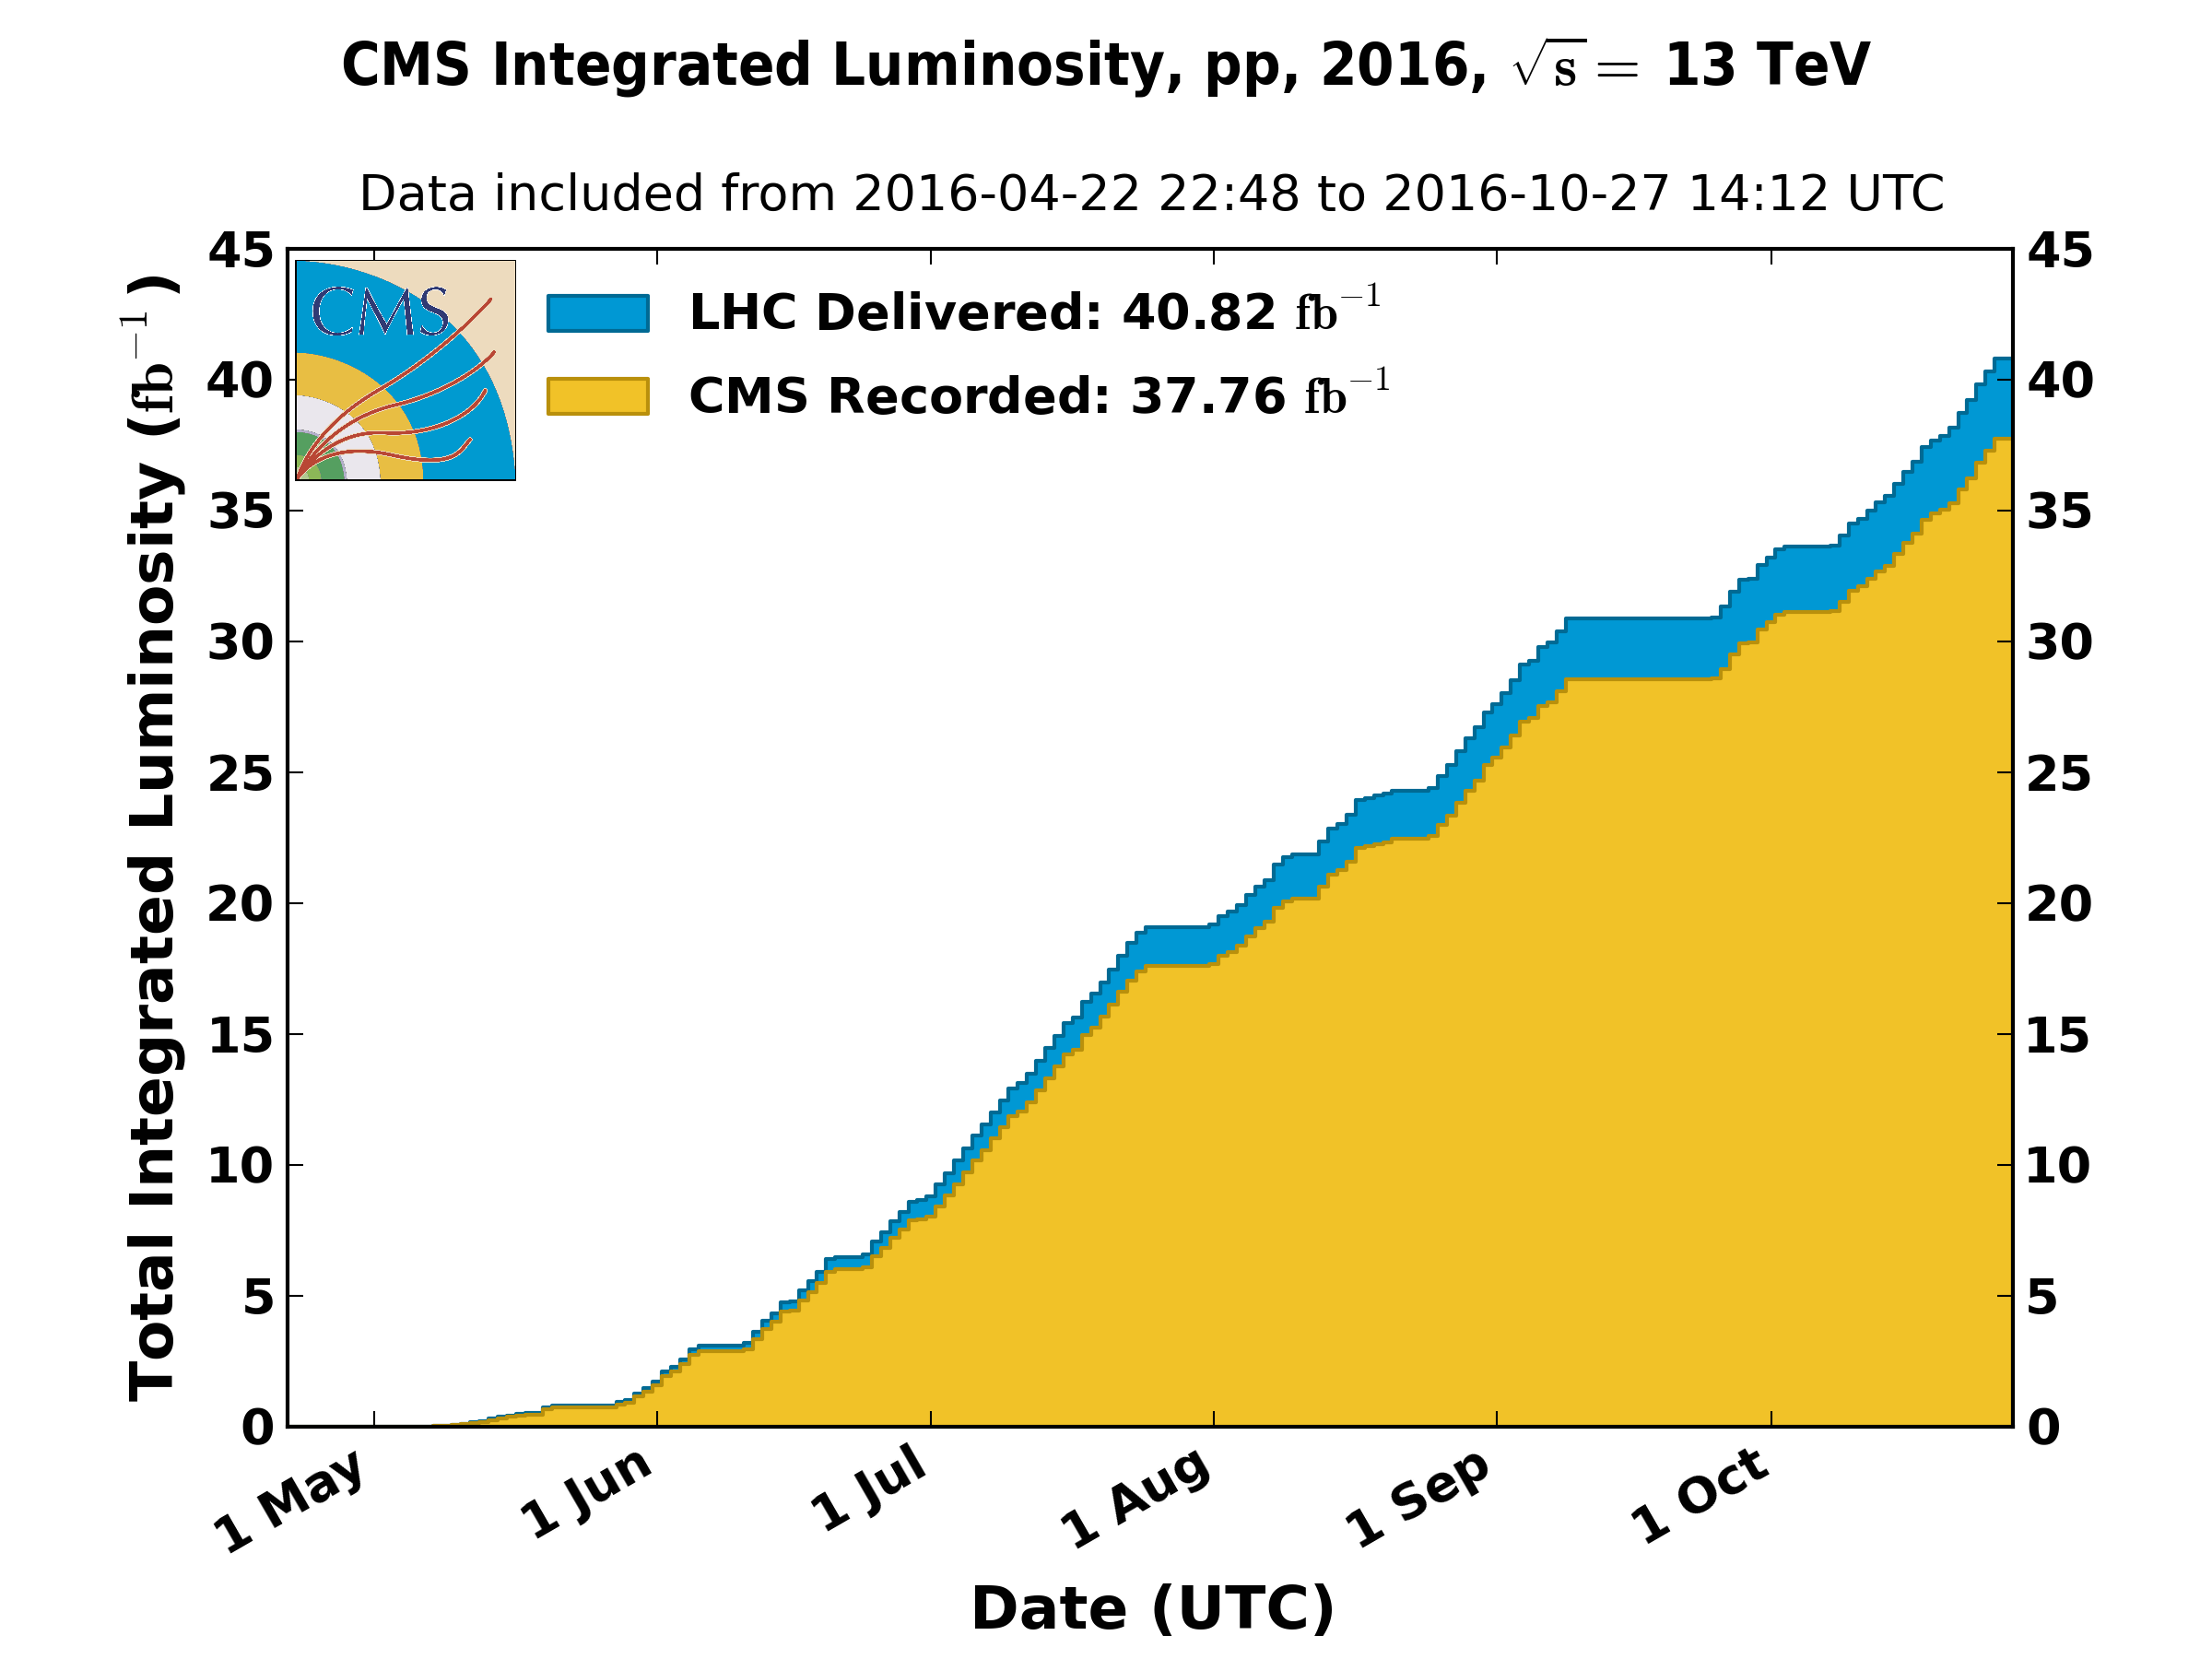
\includegraphics[width=.75\textwidth]{CMS_recorded_lumi}
 \caption{The cumulative distribution of the instantaneous luminosity delivered by the \ac{LHC} (blue) and recorded by \ac{CMS} (yellow) in 2016.}
 \label{fig:CMSlumi}
\end{figure}

\subsubsection{Pre-amplifier saturation in the APV25 chip}

During Run 2, the instantaneous luminosity delivered by the \ac{LHC} increased continuously, and even exceeded the design luminosity of $10^{34}$ cm$^{-2}$s$^{-1}$ in 2016. As the luminosity increased, a dynamic inefficiency appeared in the strip tracker, which was most noticeable in the first layer of the \ac{TOB}. The symptoms were a change in the signal-to-noise ratio and loss of hits. As can be seen from Figure~\ref{fig:SOverN}, the most probable value (MPV) of the signal-to-noise ratio is shifted towards lower values and the low tail increased as well. The loss of hits is clearly visible in Figure~\ref{fig:nhits}, showing the change in number of hits per track for increasing instantaneous luminosities. The run periods indicated in the plot refer to a subset of the data taken over the course of the year. Run period boundaries are typically defined by changes in the \ac{LHC} running conditions, changes to the detector configuration or calibration, or other parameters. The number of hits decreases for later run periods such as D and F, as the instantaneous luminosity increases. This loss of hits results in less and shorter tracks.
  
\begin{figure}[ht]
  \centering
 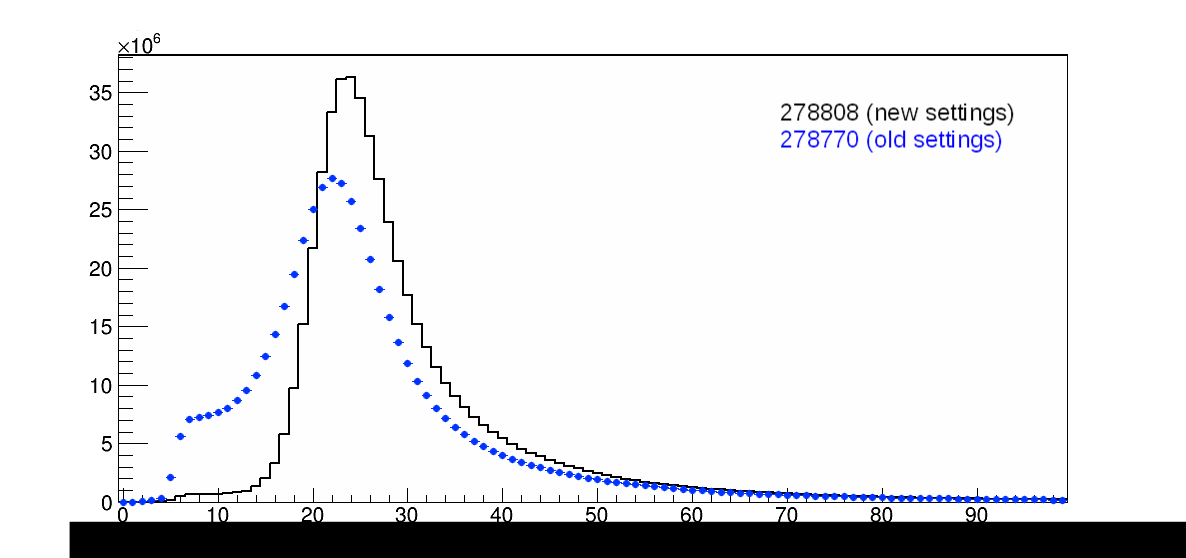
\includegraphics[width=.9\textwidth]{APVsaturation_SOverN}
 \caption{The signal-to-noise ratio for clusters on reconstructed tracks in the first layer of the \ac{TOB} for a run before (blue) and after (black) the change of pre-amplifier drain speed.}
 \label{fig:SOverN}
\end{figure}
  
\begin{figure}[ht]
  \centering
 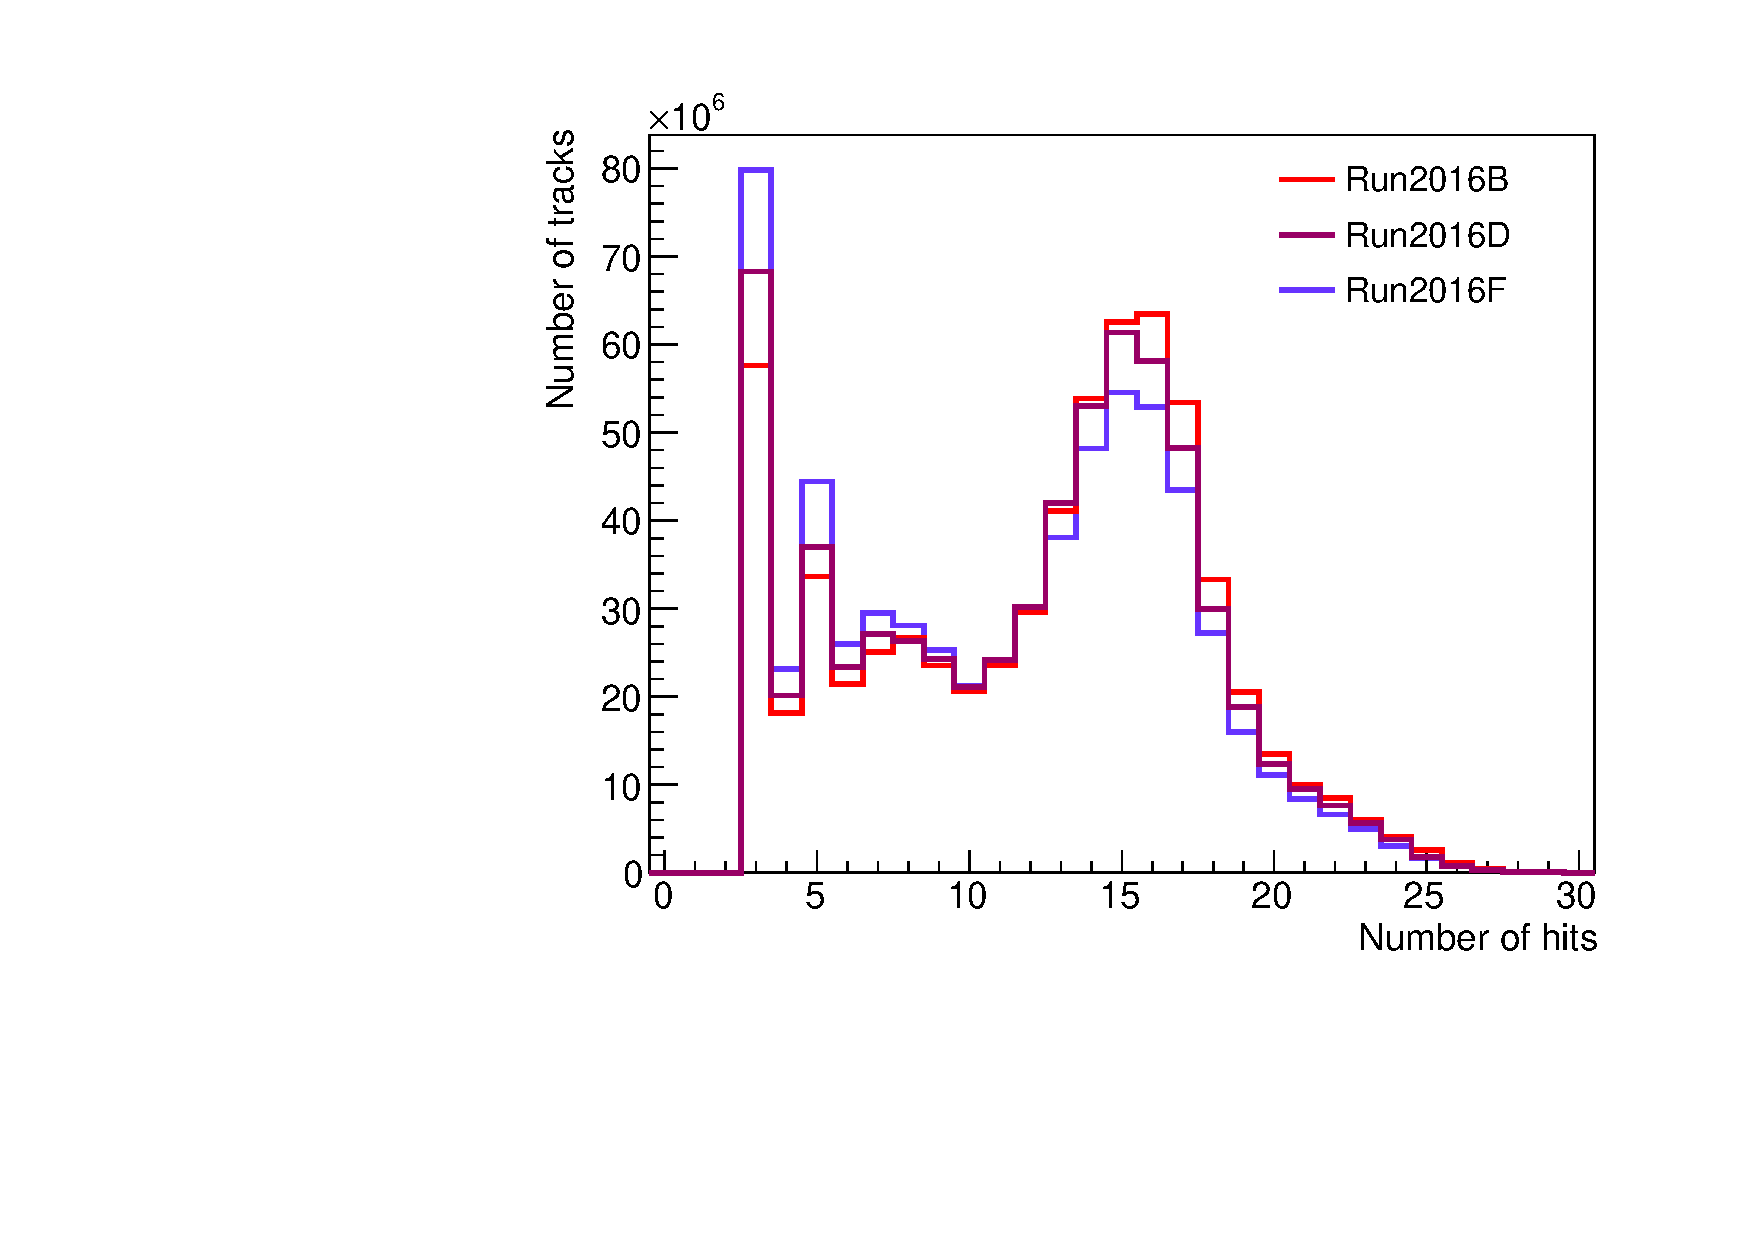
\includegraphics[width=.6\textwidth]{nhits_perRunPeriod}
%  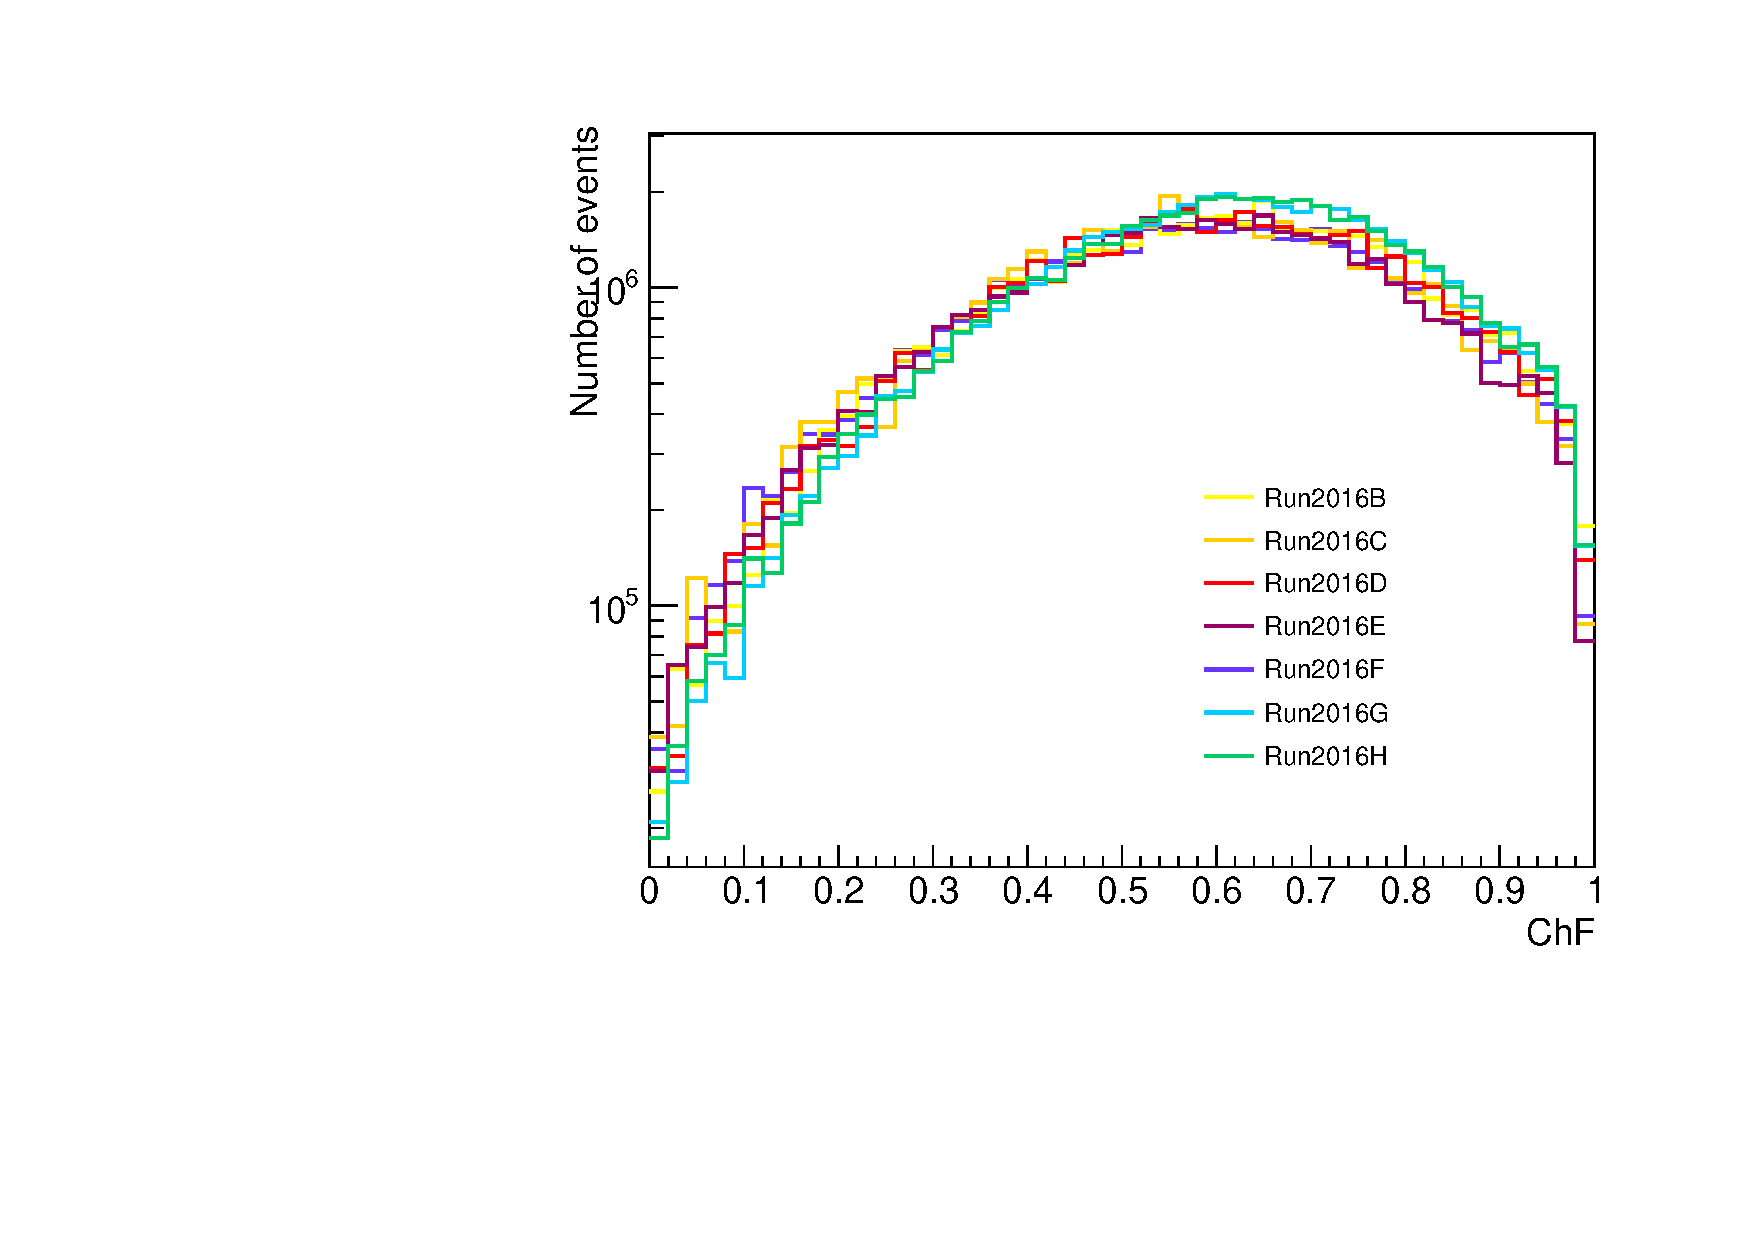
\includegraphics[width=.47\textwidth]{ChF_perRunPeriod}
 \caption{The number of hits per track for run periods B, D, and F, showing the effect of the increasing instantaneous luminosity.}
 \label{fig:nhits}
\end{figure}

The origin of this inefficiency was eventually tracked down to saturation effects in the pre-amplifier of the APV25 chip. The pre-amplifier decay time changes significantly with temperature. As the operating temperature of the strip tracker was lowered from $+4$\degree C to $-15$\degree C coolant temperature during LS1, the decay time was no longer sufficient to cope with the high luminosities. The dynamic inefficiency was cured in August 2016 by changing the pre-amplifier drain speed. This lead among others to the recovery of the muon efficiency, which showed a large drop for the highest luminosities before the change and an essentially flat behavior afterwards, as demonstrated in Figure~\ref{fig:muoneff}.
  
\begin{figure}[ht]
  \centering
 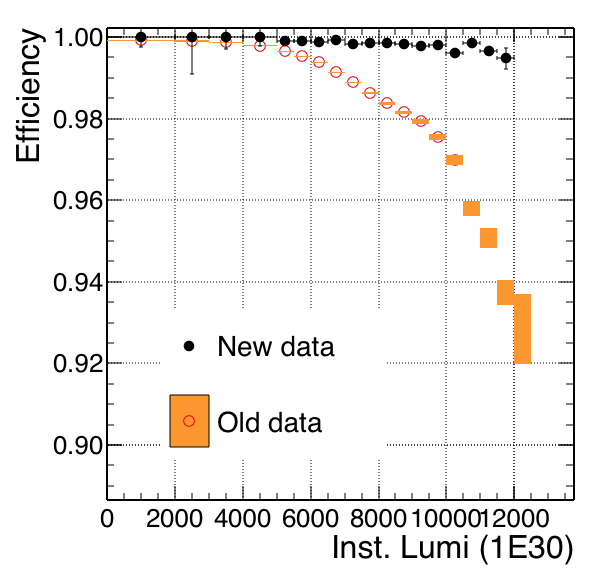
\includegraphics[width=.6\textwidth]{APVsaturation_muoneff}
 \caption{The muon efficiency as a function of the instantaneous luminosity for before (orange) and after (black) the change of pre-amplifier drain speed which cured the dynamic inefficiency.}
 \label{fig:muoneff}
\end{figure}

\clearpage

\clearpage{\pagestyle{empty}\cleardoublepage}

\graphicspath{{chapt_dutch/}{intro/}{chapt2/}{chapt3/}{chapt4/}{chapt5/}}

% Header
\renewcommand\evenpagerightmark{{\scshape\small Chapter 4}}
\renewcommand\oddpageleftmark{{\scshape\small Event Simulation and Reconstruction}}

\hyphenation{}

\chapter{Event Simulation and Reconstruction}
\label{ch4}

In order to 2 addditional tools? are needed.

\section{Event generation}

\section{Detector simulation}

\subsection{Delphes}

\subsection{GEANT4}

\section{Event reconstruction}

\subsection{Track reconstruction}

The tracks of charged particles going through the \ac{CMS} tracker are reconstructed with an iterative tracking approach. This is used to cope with the high occupancy and consequently high combinatorics. Additionally, the first iterations search for tracks with less possible combinations, such as tracks with many pixel hits or a high momentum. After every iteration, the hits associated with the found track are removed to reduce the combinatorics. Each iteration consists of four steps:
\begin{enumerate}
 \item \textbf{Seed generation.} In this first step hits are combined into seeds for the subsequent track finding. In the initial iterations pixel triplets are used, then pixel pairs, in order to take gaps or non-working modules into account. Next, mixed pixel/strip triplets are taken, and finally strip-only seeds are used. These additional iterations improve the acceptance in $p_T$ and in displacement with respect to the primary vertex.
 \item \textbf{Track finding}. The seeds are used as starting point for a Kalman filter algorithm. This method extrapolates the seed trajectory outward to the next layer, taking into account potential energy loss and multiple scattering. If compatible hits are found in the next layer, the parameters of the trajectory are updated. This process continues until the outermost layer of the tracking system. Using this method, a given seed can generate multiple tracks, or different tracks can share hits. A trajectory cleaner therefore determines the fraction of hits the tracks have in common and discards the track with the lowest number of hits when there are too many shared hits. If both tracks have the same number of hits, the track with the largest $\chi^2$ value is removed.
 \item \textbf{Track fitting.} The track parameters are then refitted using a Kalman filter and smoother, taking all hits determined in the track finding step into account.
 \item \textbf{Track selection.} Finally, the tracks are selected based on quality requirements, such as the number of layers that have hits, the $\chi^2/$dof, and the distance to a primary vertex. This greatly reduces the fraction of reconstructed tracks that are fake.
\end{enumerate}

The performance of the track reconstruction is excellent, and a high track-finding efficiency is obtained~\cite{Chatrchyan:2014fea} while keeping the rate of fake tracks negligible. The highest tracking efficiency is obtained for muons, which traverse the full detector volume and have an improved momentum resolution due to tracking information from the muon detectors giving a long lever arm. For isolated muons with $p_T$ between 1 and \SI{100}{GeV} the tracking efficiency is higher than 99\% for the entire $\eta$ coverage of the tracker, as can be seen from the left plot in Figure~\ref{fig:eff_eta}. The $p_T$ resolution is about 2-3\% for a muon with $p_T = $ \SI{100}{GeV} up to $|\eta| < 1.6$, but worsens for higher pseudorapidities. Different types of particles interact differently with the detector material. Charged hadrons, for example, are also subject to elastic and inelastic nuclear interactions and have a tracking efficiency of 80-95\% depending on pseudorapidity and transverse momentum, as shown in the right plot of Figure~\ref{fig:eff_eta}.

\begin{figure}[ht]
  \centering
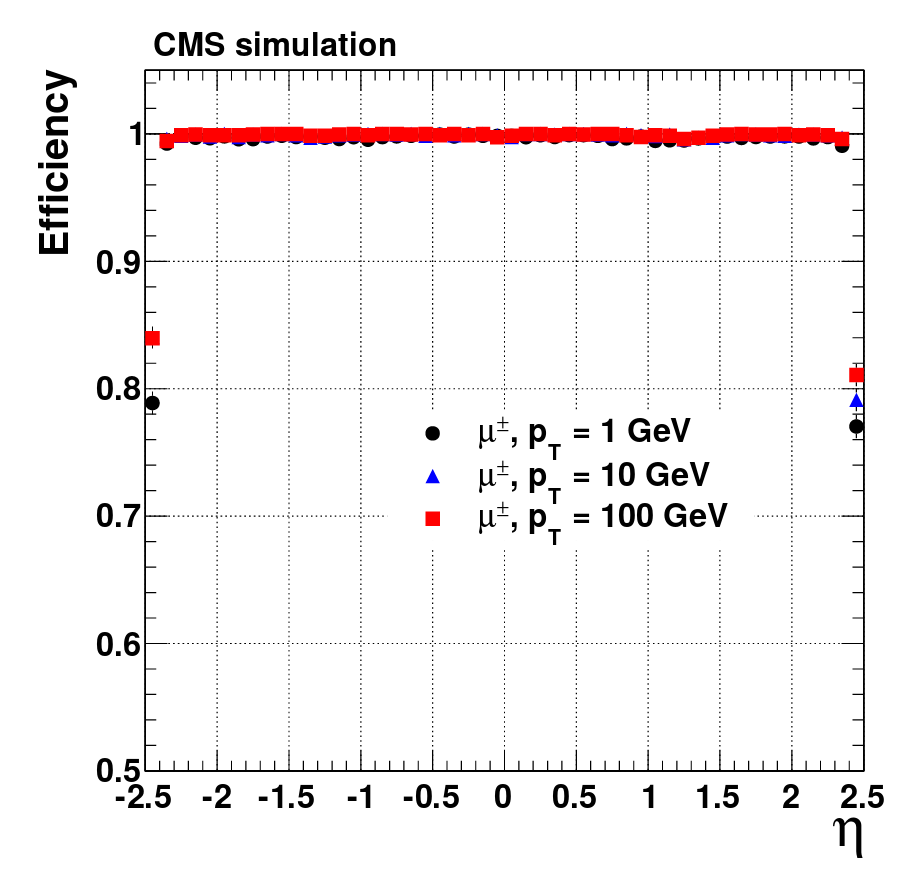
\includegraphics[width=.4\textwidth]{muon_eff_eta}\hspace{1cm}
 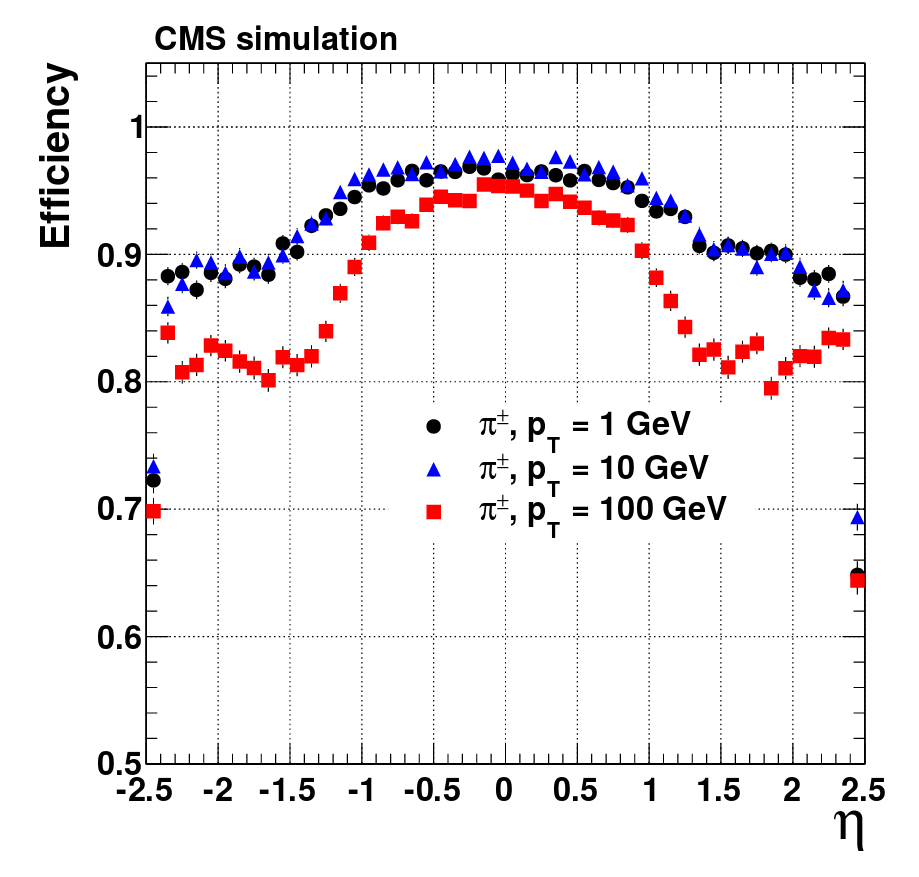
\includegraphics[width=.4\textwidth]{pion_eff_eta} 
 \caption{The muon efficiency (left) and pion efficiency (right) as a function of pseudorapidity, for multiple transverse momenta.~\cite{Chatrchyan:2014fea}}
 \label{fig:eff_eta}
\end{figure}

Finally, the primary vertex is reconstructed from the tracks. Since the collisions happen between bunches of protons, multiple protons will be colliding at the same time. The extra collisions, next to the potentially interesting collision, are referred to as pile-up interactions. The particles generated in these collisions are all detected simultaneously and form a challenge to disentangle them from the particles coming from the to be studied interaction.

The reconstruction is done in 2 steps: first the tracks that appear to originate from the same interaction vertex are clustered, then a fitting procedure computes the vertex parameters and assigns a weight to each associated track, reflecting the probability that it corresponds to the considered vertex. Figure~\ref{fig:PV} shows the reconstruction efficiency and the resolution of the primary vertex. The more tracks, the better the vertex is constrained and thus the better the resolution.

\begin{figure}[ht]
  \centering
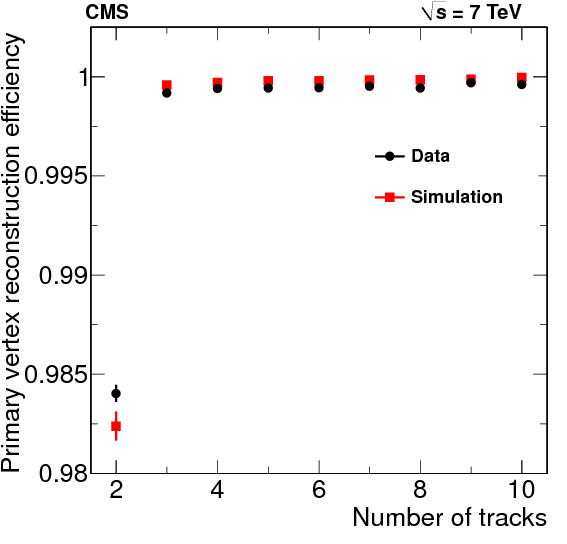
\includegraphics[width=.4\textwidth]{PV_eff}\hspace{1cm}
 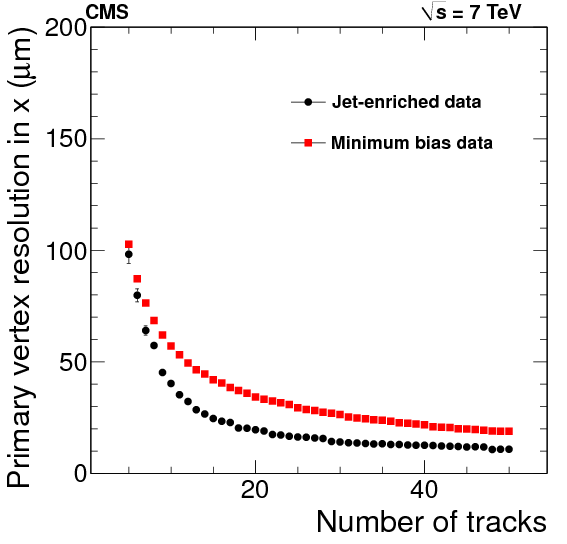
\includegraphics[width=.4\textwidth]{PV_res} 
 \caption{The primary vertex reconstruction efficiency (left) and resolution (right) as a function of the number of tracks associated to it.~\cite{Chatrchyan:2014fea}}
 \label{fig:PV}
\end{figure}

\subsection{Electron and isolated photon reconstruction}
\label{sec:electron_reconstruction}

Electrons are reconstructed using information from both the tracker and the calorimeters. Due to the large amount of material present in the tracker, electrons will emit bremsstrahlung photons, and photons will often convert into $e^+e^-$ pairs, which can again radiate bremsstrahlung photons. The electron and photon reconstruction is therefore very similar.

For electrons, a \ac{GSF} candidate is taken as starting point. This candidate is obtained using 2 different methods to reconstruct the electron track from the hits in the tracker. This track reconstruction should gather all radiated energy from the electron. First, the ECAL-based approach is used, grouping \ac{ECAL} clusters into superclusters. These superclusters collect the energy of the electron and the bremsstrahlung photons in a small $\eta$ window and a large $\phi$ window, taking the bending of the electron in the magnetic field into account. The supercluster energy and position is then used to determine the position of the corresponding hits in the tracker layers. Next, the tracker-based approach is used to reconstruct electrons missed by the ECAL-based method. In this case, all the tracks from the iterative tracking with transverse momentum larger than \SI{2}{GeV} are used. The obtained electron seeds are then used in the specific electron tracking, done by a \ac{GSF} fit, which is more adapted to electrons than the Kalman filter used in the iterative tracking, as it describes the energy loss in each tracker layer. In the case of isolated photons, a candidate is seeded from an \ac{ECAL} supercluster with transverse energy larger than \SI{10}{GeV} which is not linked to a \ac{GSF} track.

The total energy of the accumulated \ac{ECAL} clusters is corrected for the energy that was lost in the process, using analytical functions of the energy and pseudorapidity. The applied corrections can be as large as 25\%, at low transverse momentum and at $|\eta| = 1.5$, where the material density in the tracker is largest. The energy of the electron is then obtained from a combination of the corrected energy and the momentum of the \ac{GSF} track, while the direction of the electron is taken from the \ac{GSF} track. For photons, the corrected energy and the direction of the supercluster are used.

Additionally, the electron and photon candidates must satisfy identification criteria to be retained. In the case of electrons a boosted decision tree is used, combining fourteen variables including the amount of energy radiated and the ratio between the energies gathered in HCAL and ECAL, while for photons the candidates must be isolated from other tracks and calorimeter clusters, and the energy distribution in the \ac{ECAL} and the ratio between the \ac{HCAL} and \ac{ECAL} energies must be compatible with the expectation from a photon shower.

\subsection{Muon reconstruction}
\label{sec:muon_reconstruction}

Muon tracking is performed using 2 complementary approaches. The first method starts from standalone muons which are reconstructed from hits in the muon detectors using pattern recognition. The standalone muons are then matched to tracks in the tracker, and the hits are combined to form a global muon track. This global muon fit improves the momentum resolution compared to the tracker-only fit at muon momenta larger than \SI{200}{GeV}.

For momenta below \SI{10}{GeV}, muons often fail the global muon conditions which require the muon to penetrate through more than one muon detector plane, due to the large multiple scattering in the return yoke. In this case, tracker muon reconstruction is more efficient since it only requires one muon segment. Each track in the tracker with a transverse momentum larger than \SI{0.5}{GeV} and a total momentum larger than \SI{2.5}{GeV} is therefore extrapolated to the muon system and if at least one matching track segment it found, it is retained as muon track.

Within the geometrical acceptance of the muon system about 99\% of the muons are reconstructed, either as global muon or as tracker muon and frequently as both. Global and tracker muons that share the same track inside the tracker are merged into a single candidate. Some muons are only reconstructed as standalone muons, in which case they have a worse momentum resolution compared to the global and tracker muons.

Charged hadrons can be misreconstructed as muons if e.g. a part of the hadron shower reaches the muon system. In order to improve the muon identification, the \ac{PF} muon identification algorithm described in Section~\ref{sec:PF} also matches energy deposits in the \ac{ECAL} and \ac{HCAL} with the muon track.

\subsection{Jet reconstruction}
\label{sec:jet_reconstruction}



\subsection{B-tagging}



\subsection{Missing transverse energy reconstruction}



\subsection{Particle flow}
\label{sec:PF}



\section{Simulation of the SIMP signal}


\clearpage
\clearpage{\pagestyle{empty}\cleardoublepage}

\graphicspath{{chapt_dutch/}{intro/}{chapt2/}{chapt3/}{chapt4/}}

% Header
\renewcommand\evenpagerightmark{{\scshape\small Conclusion}}
\renewcommand\oddpageleftmark{{\scshape\small Conclusion}}

\hyphenation{}

\chapter{The Monojet Analysis}

\section{Introduction}

\section{Event selection}

\section{Background estimation}

\section{Results}

\section{Improvement going from the 2015 to 2016 analysis}

\section{Interpretation}

\clearpage{\pagestyle{empty}\cleardoublepage}

\graphicspath{{chapt_dutch/}{intro/}{chapt2/}{chapt3/}{chapt4/}{chapt5/}}

% Header
\renewcommand\evenpagerightmark{{\scshape\small Chapter 5}}
\renewcommand\oddpageleftmark{{\scshape\small Media Grids}}

\renewcommand{\bibname}{References}

\hyphenation{}

\chapter{Search for SIMPs using Trackless Jets}
\label{ch5}

\section{Introduction}

\section{Event selection}

\section{Background estimation}

\section{Results}

\section{SIMP model interpretation}

\clearpage


\clearpage{\pagestyle{empty}\cleardoublepage}

\graphicspath{{chapt_dutch/}{intro/}{chapt2/}{chapt3/}{chapt4/}}

% Header
\renewcommand\evenpagerightmark{{\scshape\small Conclusion}}
\renewcommand\oddpageleftmark{{\scshape\small Conclusion}}

\hyphenation{}

\chapter{Conclusion \& Outlook}



%\renewcommand*{\thesection}{\thechapter.\arabic{section}}       % reset again to chaptnum.sectnum

\clearpage{\pagestyle{empty}\cleardoublepage}


\clearpage

\bibliographystyle{phdbib}
\bibliography{PhD}


%\addcontentsline{toc}{section}{}

% \appendix
% \graphicspath{{chapt_dutch/}{intro/}{chapt2/}{chapt3/}{chapt4/}{chapt5/}}

% Header
\renewcommand\evenpagerightmark{{\scshape\small Appendix A}}
\renewcommand\oddpageleftmark{{\scshape\small Grid Computing: The Next Network Challenge!}}

\renewcommand{\bibname}{References}

\hyphenation{}

\chapter[Grid Computing: The Next Network Challenge!]%
{Grid Computing: The Next Network Challenge!}
\label{app1}

\par{\large{\textbf{B. Volckaert, P. Thysebaert, M. De Leenheer, F. De Turck, B. Dhoedt, P. Demeester}}}
\vspace{0.2in}
\par{\noindent\textbf{published in The Journal of The Communications Network (Proceedings of FITCE 2004), 43rd European Telecommunications Congress, 2004, Vol. 3, pp. 159-165.}}
\vspace{0.1in}

\par{\bf{Abstract}}
\emph{
abstract
}

\section{Introduction}
Start text here...

\bibliographystyle{phdbib}
\bibliography{PhD}

\clearpage{\pagestyle{empty}\cleardoublepage}

% \newfloat{algo}{h}{alg}

\graphicspath{{chapt_dutch/}{intro/}{chapt2/}{chapt3/}{chapt4/}{chapt5/}}

% Header
\renewcommand\evenpagerightmark{{\scshape\small Appendix B}}
\renewcommand\oddpageleftmark{{\scshape\small Application-specific hints in reconfigurable Grid scheduling algorithms}}

\renewcommand{\bibname}{References}

\hyphenation{}

\chapter[Application-specific hints in reconfigurable Grid scheduling algorithms]%
{Application-specific hints in reconfigurable Grid scheduling algorithms}
\label{app2}

\par{\large{\textbf{B. Volckaert, P. Thysebaert, F. De Turck, B. Dhoedt, P. Demeester}}}
\vspace{0.2in}
\par{\noindent\textbf{published in Lecture Notes in Computer Science (LNCS 3038), Computational Science, Proceedings P3 of ICCS 2004, Springer-Verlag Berlin Heidelberg 2004, Krakow, 2004, Vol. LNCS 3038, pp. 149-157.}}
\vspace{0.1in}

\par{\bf{Abstract}}
\emph{
abstract...
}


\section{Introduction}
insert text here

\bibliographystyle{phdbib}
\bibliography{PhD}

\clearpage{\pagestyle{empty}\cleardoublepage}
% \graphicspath{{chapt_dutch/}{intro/}{chapt2/}{chapt3/}{chapt4/}{chapt5/}}

% Header
\renewcommand\evenpagerightmark{{\scshape\small Appendix C}}
\renewcommand\oddpageleftmark{{\scshape\small Network Aware Scheduling in Grids}}

\renewcommand{\bibname}{References}

\hyphenation{}

\chapter[Network Aware Scheduling in Grids]%
{Network Aware Scheduling in Grids}
\label{app3}

\par{\large{\textbf{B. Volckaert, P. Thysebaert, M. De Leenheer, F. De Turck, B. Dhoedt, P. Demeester}}}
\vspace{0.2in}
\par{\noindent\textbf{published in Proceedings of NOC2004, 9th European Conference on Networks \& Optical Communications, TU Eindhoven, 2004, pp. 311-318.}}
\vspace{0.1in}

\par{\bf{Abstract}}
\emph{
abstract
}

\section{Introduction}
insert text here...

\bibliographystyle{phdbib}
\bibliography{PhD}

\clearpage{\pagestyle{empty}\cleardoublepage}


%\renewcommand\fdtsvrightmarktmp{{\scshape\small Appendix }}
\renewcommand\evenpagerightmark{{\scshape\small Appendix \thechapter}}
\renewcommand\oddpageleftmark{{\scshape\small\leftmark}}


% \listoffigures
% \clearpage{\pagestyle{empty}\cleardoublepage}
% 
% \listoftables
% \clearpage{\pagestyle{empty}\cleardoublepage}

% List of Acronyms
%%%%%%%%%%%%%%%%%%%%%%%%%%%%%%%%%%%%%%%%%%%%%%%%%%%%%%%%%%%%%%%%%%%%%

\chapter*{List of Acronyms}
%     \@mkboth{\MakeUppercase List of Acronyms}%
%              {\MakeUppercase List of Acronyms}%

%\begin{center}
%\textbf{\Large List of Acronyms}
%\end{center}
\textbf{\newline\newline\Large A} \newline
\begin{acronym_expdlist}
\acro{ATLAS}{A Toroidal LHC ApparatuS}
\end{acronym_expdlist}

\textbf{\newline\newline\Large B} \newline
\begin{acronym_expdlist}
\acro{BU}{Builder Unit}
\end{acronym_expdlist}
% 
\textbf{\newline\newline\Large C} \newline
\begin{acronym_expdlist}
\acro{CERN}{European Organization for Nuclear Research}
\acro{CMS}{Compact Muon Solenoid}
\acro{CSC}{Cathode Strip Chambers}
\end{acronym_expdlist}
% 
\textbf{\newline\newline\Large D} \newline
\begin{acronym_expdlist}
\acro{DAQ}{data acquisition}
\acro{DQM}{Data Quality Monitoring}
\acro{DT}{Drift Tubes}
\end{acronym_expdlist}
% 
\textbf{\newline\newline\Large E} \newline
\begin{acronym_expdlist}
\acro{ECAL}{electromagnetic calorimeter}
\end{acronym_expdlist}
% 
\textbf{\newline\newline\Large F} \newline
\begin{acronym_expdlist}
\acro{FED}{Front End Driver}
\acro{FSR}{final state radiation}
\acro{FU}{Filter Unit}
\end{acronym_expdlist}

\textbf{\newline\newline\Large G} \newline
\begin{acronym_expdlist}
\acro{GSF}{Gaussian-sum filter}
\end{acronym_expdlist}

\textbf{\newline\newline\Large H} \newline
\begin{acronym_expdlist}
\acro{HCAL}{hadronic calorimeter}
\acro{HLT}{High-Level Trigger}
\end{acronym_expdlist}
% 
\textbf{\newline\newline\Large I} \newline
\begin{acronym_expdlist}
\acro{IP}{interaction point}
\acro{ISR}{initial state radiation}
\end{acronym_expdlist}

\textbf{\newline\newline\Large J} \newline
\begin{acronym_expdlist}
\acro{JER}{jet energy resolution}
\end{acronym_expdlist}

%\textbf{\newline\newline\Large K} \newline
%\begin{acronym_expdlist}
%\end{acronym_expdlist}

\textbf{\newline\newline\Large L} \newline
\begin{acronym_expdlist}
\acro{L1}{Level-1}
\acro{LEIR}{Low Energy Ion Ring}
\acro{LEP}{Large Electron Positron}
\acro{LHC}{Large Hadron Collider}
\acro{LO}{leading order}
\end{acronym_expdlist}

% \textbf{\newline\newline\Large M} \newline
% \begin{acronym_expdlist}
% \end{acronym_expdlist}
% 
\textbf{\newline\newline\Large N} \newline
\begin{acronym_expdlist}
\acro{NLO}{next-to-leading order}
\end{acronym_expdlist}
% 
% \textbf{\newline\newline\Large O} \newline
% \begin{acronym_expdlist}
% \end{acronym_expdlist}
% 
\textbf{\newline\newline\Large P} \newline
\begin{acronym_expdlist}
\acro{PDF}{parton distribution function}
\acro{PF}{particle flow}
\acro{PS}{Proton Synchrotron}
\acro{PSB}{Proton Synchrotron Booster}
\end{acronym_expdlist}

\textbf{\newline\newline\Large Q} \newline
\begin{acronym_expdlist}
\acro{QCD}{Quantum Chromodynamics}
\end{acronym_expdlist}

\textbf{\newline\newline\Large R} \newline
\begin{acronym_expdlist}
\acro{RF}{radio-frequency}
\acro{ROC}{read-out chip}
\acro{RPC}{Resistive Plate Chambers}
\acro{RU}{Readout Unit}
\end{acronym_expdlist}
% 
\textbf{\newline\newline\Large S} \newline
\begin{acronym_expdlist}
\acro{SIMP}{strongly interacting massive particle}
\acro{SPS}{Super Proton Synchrotron}
\end{acronym_expdlist}
% 
\textbf{\newline\newline\Large T} \newline
\begin{acronym_expdlist}
\acro{TEC}{Tracker EndCaps}
\acro{TIB}{Tracker Inner Barrel}
\acro{TID}{Tracker Inner Disks}
\acro{TOB}{Tracker Outer Barrel}
\end{acronym_expdlist}
% 
% \textbf{\newline\newline\Large U} \newline
% \begin{acronym_expdlist}
% \end{acronym_expdlist}
% 
% \textbf{\newline\newline\Large V} \newline
% \begin{acronym_expdlist}
% \end{acronym_expdlist}
% 
% \textbf{\newline\newline\Large W} \newline
% \begin{acronym_expdlist}
% \end{acronym_expdlist}
% 
% \textbf{\newline\newline\Large X} \newline
% \begin{acronym_expdlist}
% \end{acronym_expdlist}

%\textbf{\newline\newline\Large Y} \newline
%\begin{acronym_expdlist}
%\end{acronym_expdlist}

%\textbf{\newline\newline\Large Z} \newline
%\begin{acronym_expdlist}
%\end{acronym_expdlist}

% End of list of Acronyms
%%%%%%%%%%%%%%%%%%%%%%%%%%%%%%%%%%%%%%%%%%%%%%%%%%%%%%%%%%%%%%%%%%%%%%



\clearpage      % clear the current page
\thispagestyle{empty}   % prevent header on this (empty -> next line) page
\mbox{}         % to insert a not empty page, so that there is min. 1 blank page before next chapter
\clearpage{\pagestyle{empty}\cleardoublepage}   % clear the current page and start on the right side

%\renewcommand{\tablename}{Table}

\renewcommand{\bibname}{References}     % instead of Bibliography
%\renewcommand\citeform{\thechapter.}
%\addcontentsline{toc}{section}{\listfigurename}   % not really sure

\end{document}